\section{Fase 4: Análisis Exploratorio de datos oncológicos}

En esta fase, el científico de datos obtiene el conjunto de datos o imágenes que fueron organizados previamente por el ingeniero de datos y realiza un \textit{Análisis exploratorio de datos} para descubrir patrones generales en la información generada. Cabe resaltar, que en esta fase el acompañamiento del médico experto en oncología es de vital importancia, ya que los datos o imágenes que van ser explorados por el científico pueden contener variables que pueden tener o no un valor significativo para el experto, ayudando así a determinar si el análisis planteado para responder la pregunta va o no por un buen camino, de modo que es posible que se agreguen o eliminen diversas variables para lograr el resultado esperado. Adicionalmente, es necesario que los diversos análisis generados estén apoyados con gráficas que sean entendibles por todo el \textit{Data Analysis Team}, esto con el propósito de aportar ideas, y desde esta fase ir encontrando posibles correlaciones entre las variables oncológicas.

Se debe agregar, que en esta fase se abarcan todas las actividades para construir el conjunto de datos o imágenes que se utilizará en la siguiente etapa de modelado y ejecución. Entre las actividades se encuentran el procesamiento y transformación de datos oncológicos, en donde es necesario realizar la limpieza de datos, combinar datos de múltiples fuentes y transformar los datos en variables de valor. En esta fase, es importante el trabajo en equipo y la comunicación continua entre el ingeniero y el científico de datos para tratar los valores no válidos o faltantes, eliminar duplicados, dar un formato adecuado y combinar archivos, tablas y plataformas. Adicionalmente, el medico experto en oncología deberá proporcionar un visto bueno para proceder con la siguiente fase. Esto dado que al ser experto en el tema de dominio tiene un conocimiento más profundo de las variables o imágenes que está observando, y si existiese información innecesaria para el diagnóstico del cáncer de mama es posible depurar dicha información para que no afecte el entrenamiento y posterior ejecución del modelo de ML y DL.

Para este caso de estudio, el análisis exploratorio de datos se realizo con los registros genéticos obtenidos del conjunto de datos \textit{“Breast Invasive Carcinoma (TCGA, Cell 2015)”}.

\newpage
\subsection{Análisis parcial de datos genómicos crudos}
En primer lugar, se realizó un análisis parcial del conjunto de datos \textit{“Breast Invasive Carcinoma (TCGA, Cell 2015)”} para conocer su composición inicial(cruda) y así poder identificar los registros que deben ser eliminados, transformados ó imputados. Cabe resaltar, que esta etapa es propuesta como parte de esta investigación para los datos de tipo genómico relacionados cáncer de mama. Lo anterior, debido a que el \textit{EDA\footnote{Exploratory Data Analysis}} tradicional parte del análisis descriptivo, y en este caso los tipos de datos son obtenidos de diferentes fuentes medicas, las cuales no presentan una estructura fija ni estándar en la informacion recopilada de los pacientes que padecen esta enfermedad, por lo que seria incorrecto realizar un análisis sobre datos que dada su estructura y forma generan informacion errónea. En la figura \ref{datos_crudos} se puede observar las composición estadística unidimensional de la 110 variables, las cuales permitieron identificar el comportamiento inicial de los datos.

En la tabla \ref{dataset_Statistics} se observan la estadísticas del conjunto de datos previo a realizar la transformación e imputación de datos. 

\begin{table*}[!htb]
	\footnotesize
	\centering
	\begin{threeparttable}
		\begin{tabular}{p{0.5cm} p{7cm} p{2cm}} \toprule
			\begin{center}$N$\end{center}   
			&\begin{center}Variable\end{center}       
			&\begin{center}Estadística\end{center}  
			%------------------------------------------------------	
			\\ \hline
			1
			& Número de variables
			& $110$
			\\ \hline
			%------------------------------------------------------	
			2
			& Variables Categóricas
			& $95$
			\\ \hline
			
			%------------------------------------------------------	
			3
			& Variables Numéricas
			& $15$
			\\ \hline
			
			%------------------------------------------------------	
			4
			& Número de filas
			& 	$818$
			\\ \hline
			%------------------------------------------------------	
			5
			& Celdas faltantes
			& $37657$
			
			\\ \hline
			%------------------------------------------------------	
			6
			& Celdas faltantes (\% )
			& $41.9\%$
			
			\\ \hline
			%------------------------------------------------------	
			7
			& Filas duplicadas 
			& $0$
			
			\\ \hline
			%------------------------------------------------------	
			8
			& Filas duplicadas (\% )
			& $0.0\%$
			
			\\ \hline
			%------------------------------------------------------	
			9
			& Tamaño total en memoria
			& $3.8 mb$
			
			\\ \hline
			%------------------------------------------------------	
			10
			& Tamaño promedio de fila en la memoria
			& $	4,8 KB$
			\\ \hline	
		\end{tabular}
		\caption{Estadísticas del conjunto de datos crudos del carcinoma invasivo de mama (TCGA, Cell 2015).}
		\label{dataset_Statistics}
	\end{threeparttable}
\end{table*}

\newpage
\begin{table}
	\begin{center} 
		\caption{Análisis parcial de datos crudos realizado en el conjunto de datos del Carcinoma invasivo de mama (TCGA, Cell 2015).}
		\label{datos_crudos}
		\begin{tabular}{ |c|c|c|c| }
			\hline 
			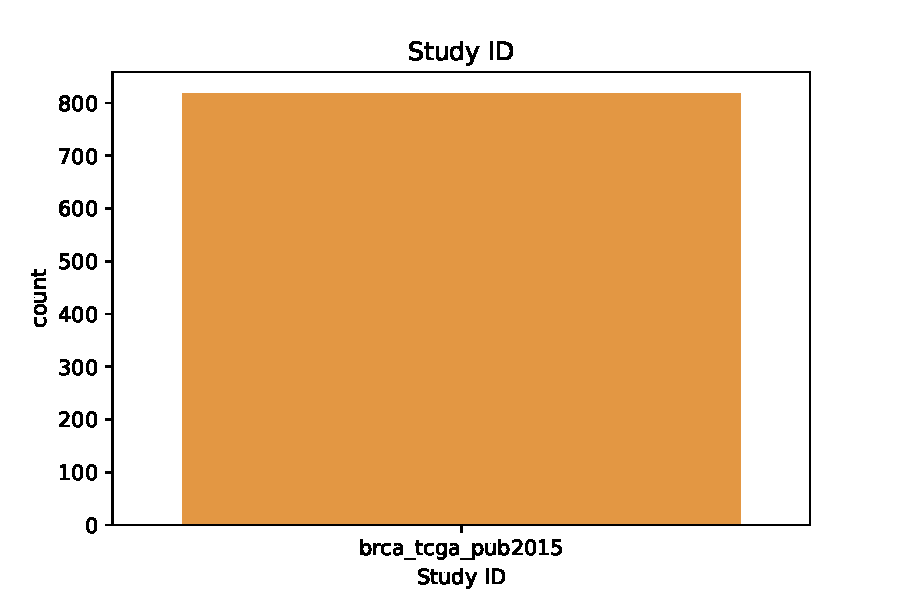
\includegraphics[width=.25\textwidth]{NOTEBOOK/IMAGENES_CRUDAS/1} 
			& 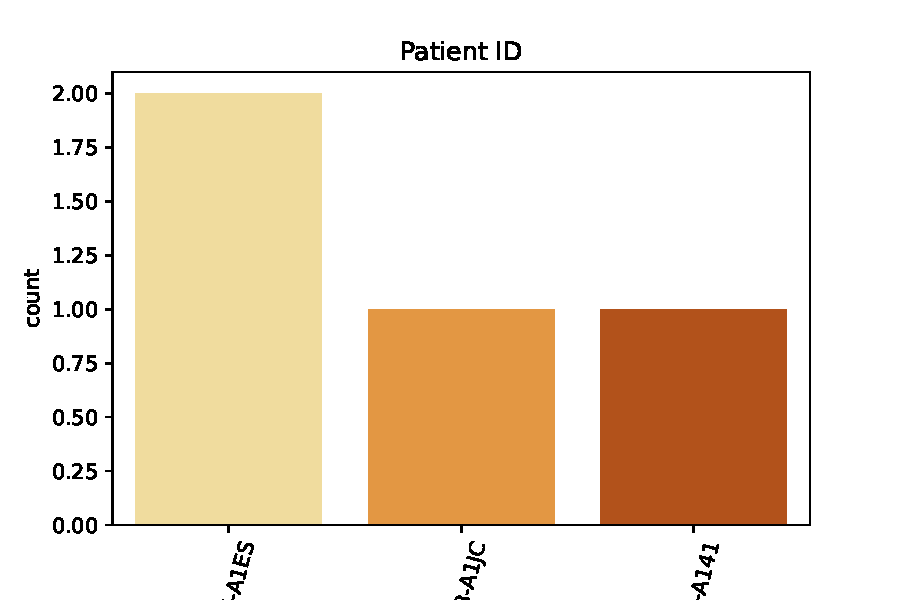
\includegraphics[width=.25\textwidth]{NOTEBOOK/IMAGENES_CRUDAS/2} 
			& 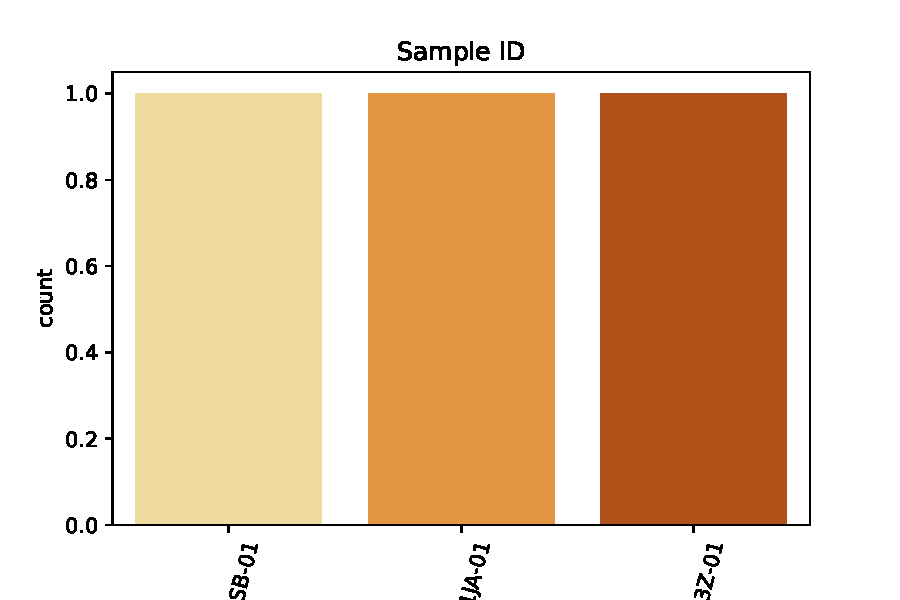
\includegraphics[width=.25\textwidth]{NOTEBOOK/IMAGENES_CRUDAS/3}
			& 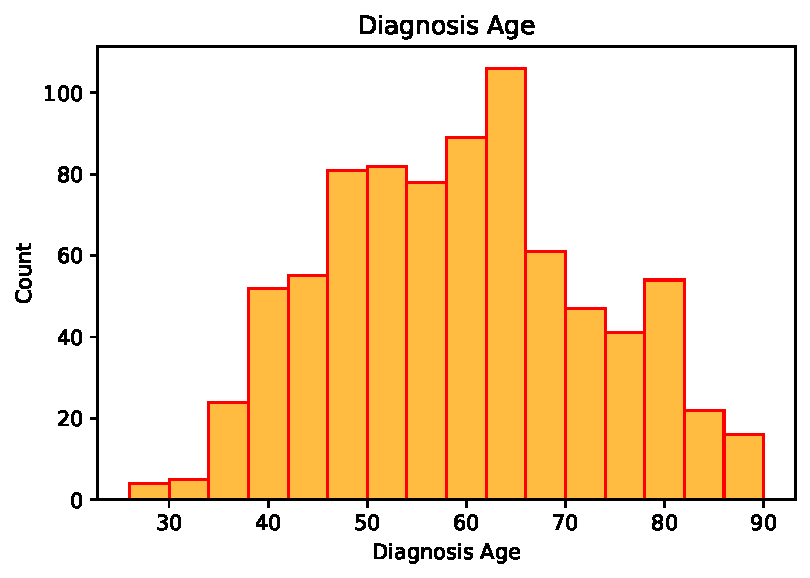
\includegraphics[width=.25\textwidth]{NOTEBOOK/IMAGENES_CRUDAS/4} 
			\\  \hline 
			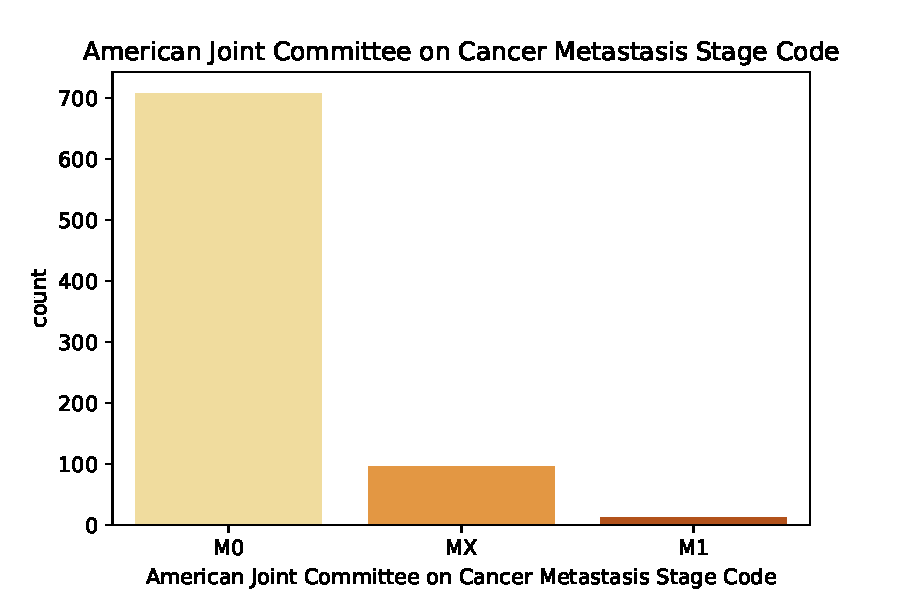
\includegraphics[width=.25\textwidth]{NOTEBOOK/IMAGENES_CRUDAS/5} 
			& 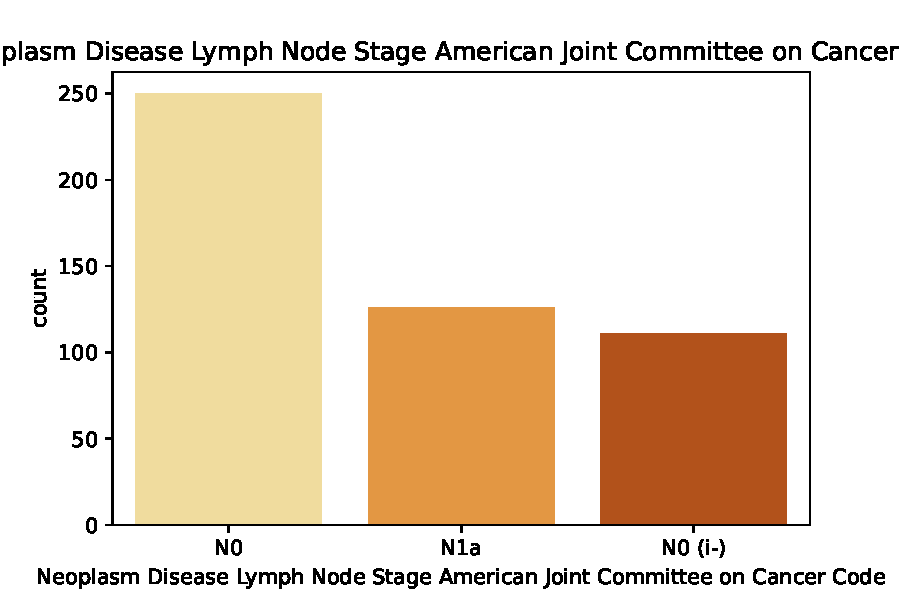
\includegraphics[width=.25\textwidth]{NOTEBOOK/IMAGENES_CRUDAS/6} 
			& 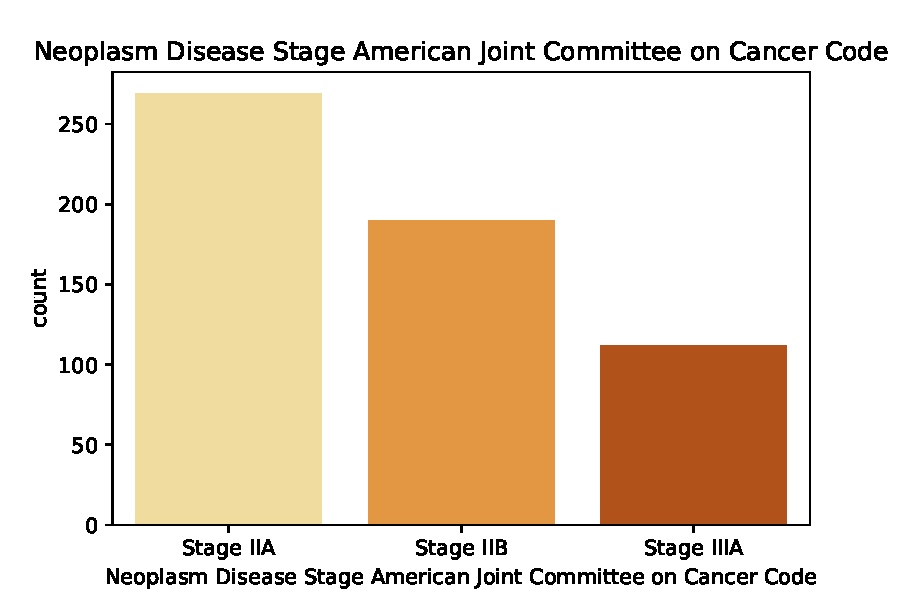
\includegraphics[width=.25\textwidth]{NOTEBOOK/IMAGENES_CRUDAS/7} 
			& 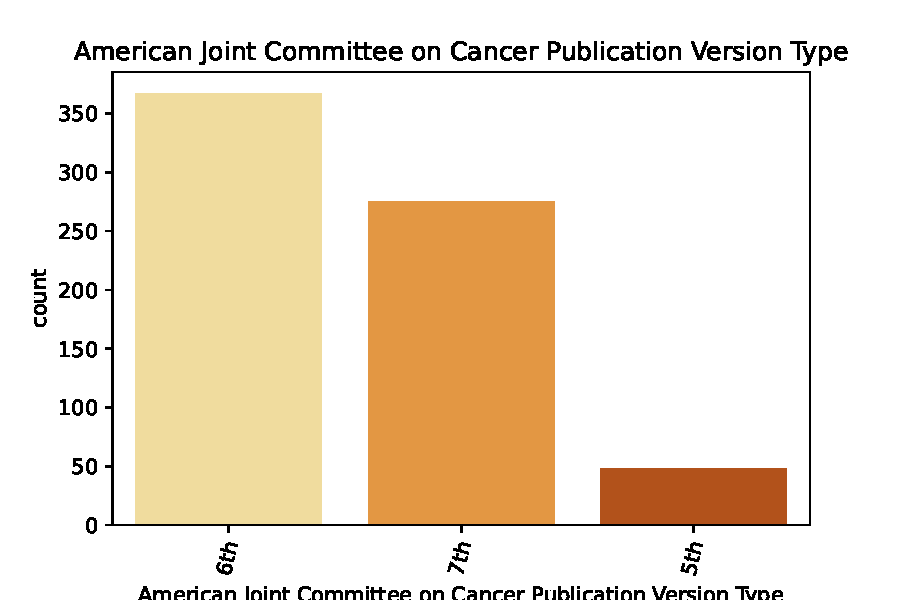
\includegraphics[width=.25\textwidth]{NOTEBOOK/IMAGENES_CRUDAS/8} 
			\\  \hline 
			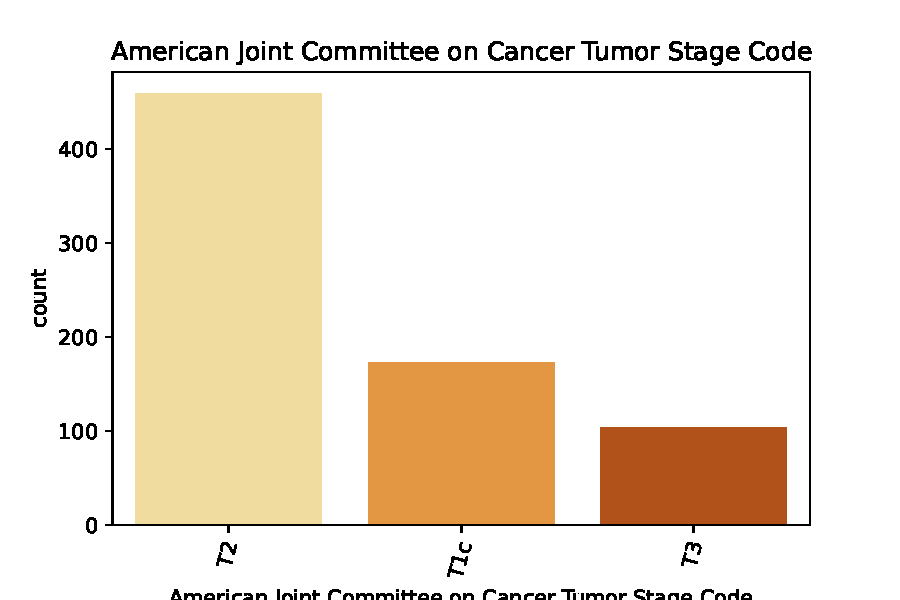
\includegraphics[width=.25\textwidth]{NOTEBOOK/IMAGENES_CRUDAS/9} 
			& 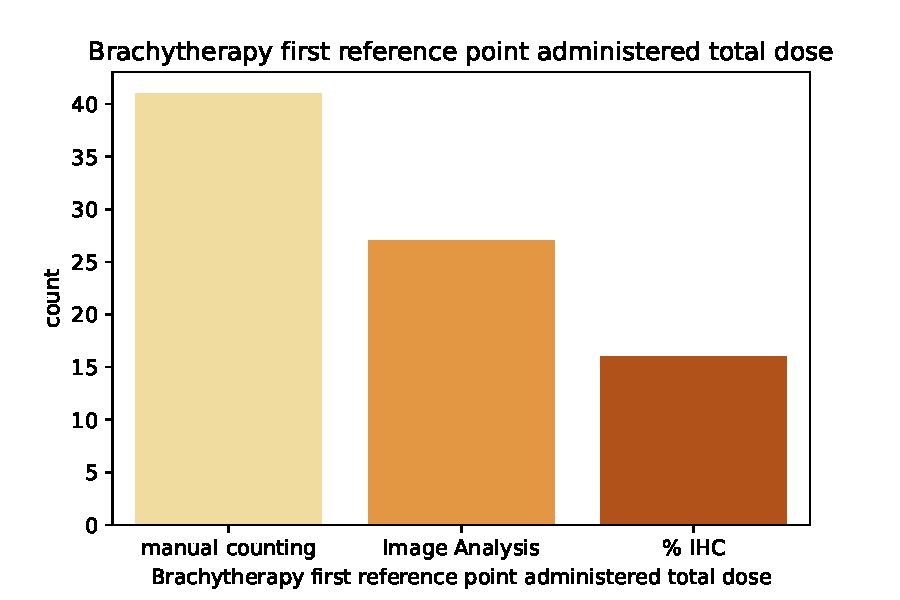
\includegraphics[width=.25\textwidth]{NOTEBOOK/IMAGENES_CRUDAS/10} 
			& 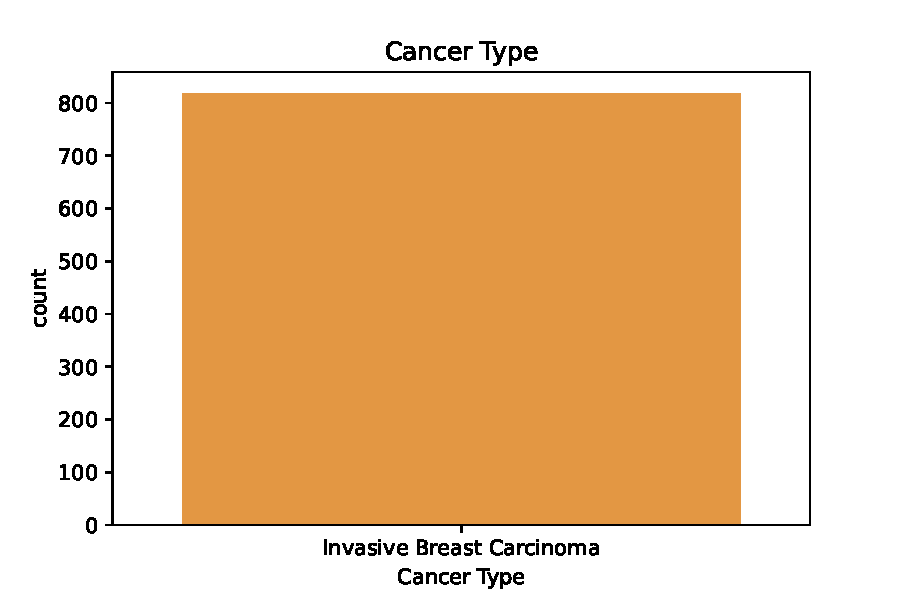
\includegraphics[width=.25\textwidth]{NOTEBOOK/IMAGENES_CRUDAS/11} 
			& 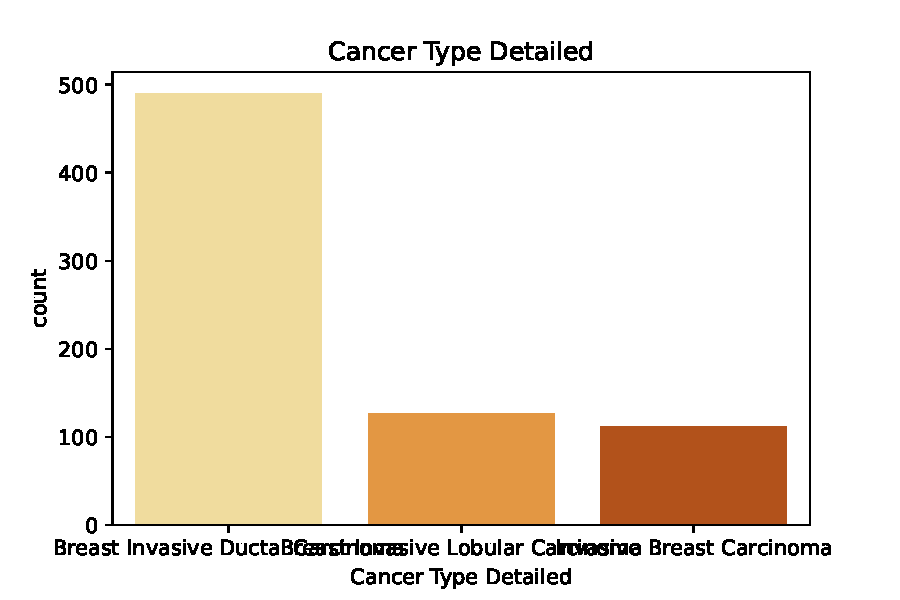
\includegraphics[width=.25\textwidth]{NOTEBOOK/IMAGENES_CRUDAS/12} 
			\\  \hline 
			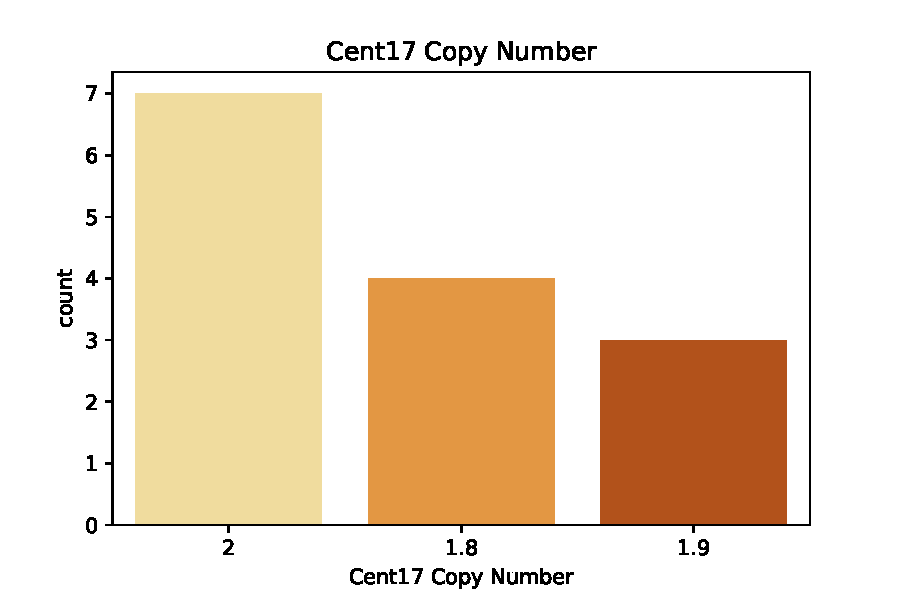
\includegraphics[width=.25\textwidth]{NOTEBOOK/IMAGENES_CRUDAS/13} 
			& 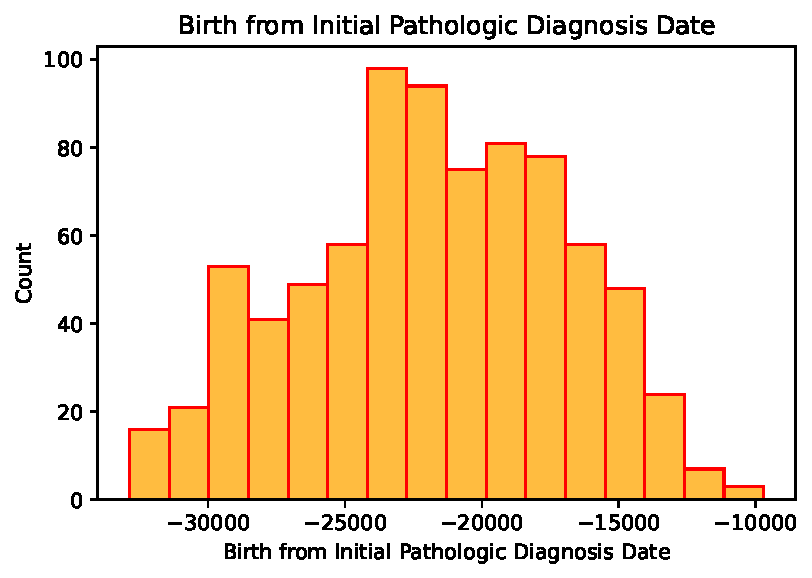
\includegraphics[width=.25\textwidth]{NOTEBOOK/IMAGENES_CRUDAS/14} 
			& 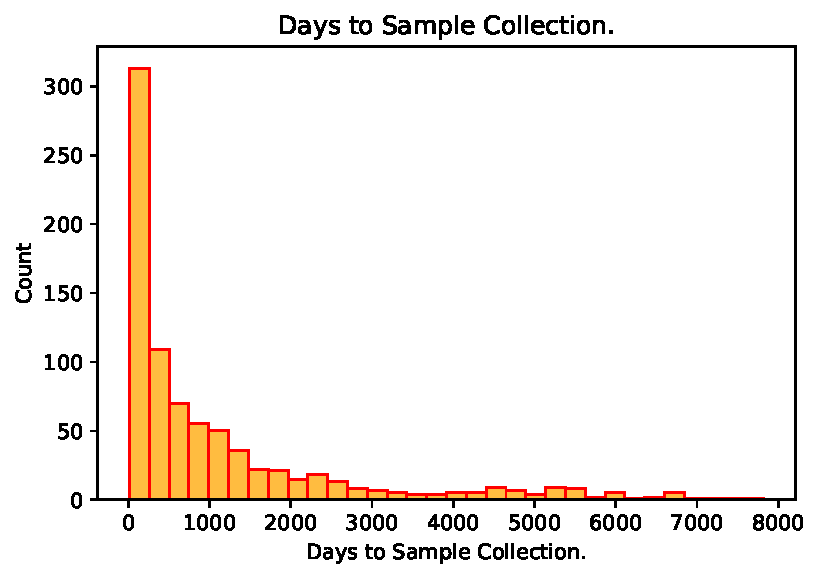
\includegraphics[width=.25\textwidth]{NOTEBOOK/IMAGENES_CRUDAS/15} 
			& 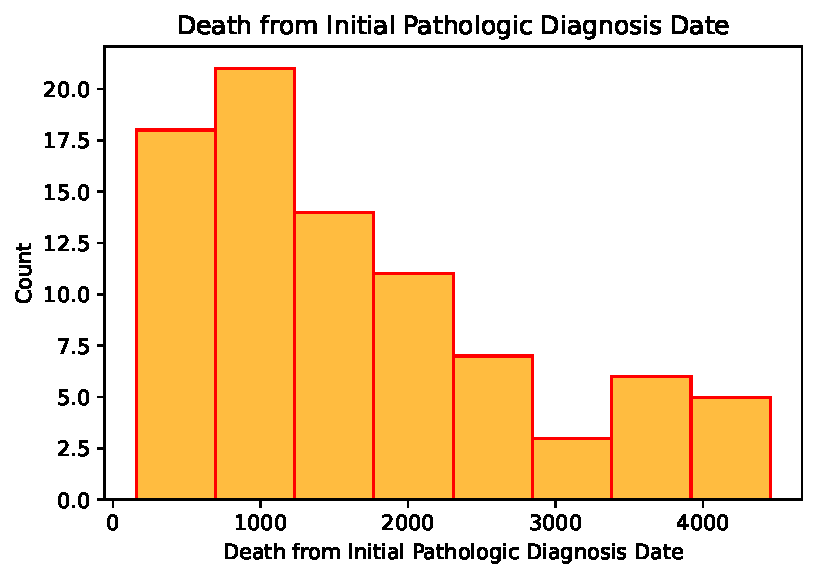
\includegraphics[width=.25\textwidth]{NOTEBOOK/IMAGENES_CRUDAS/16} 
			\\  \hline
			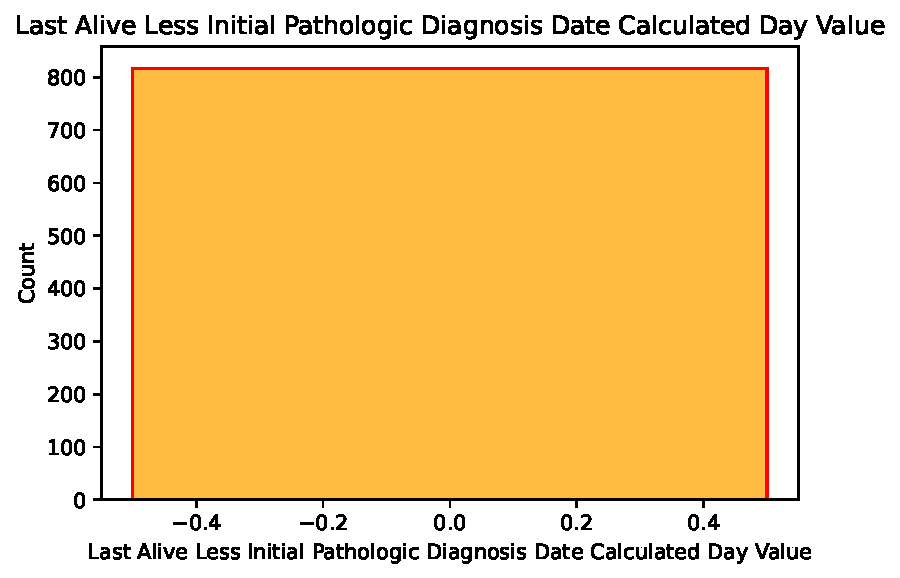
\includegraphics[width=.25\textwidth]{NOTEBOOK/IMAGENES_CRUDAS/17} 
			& 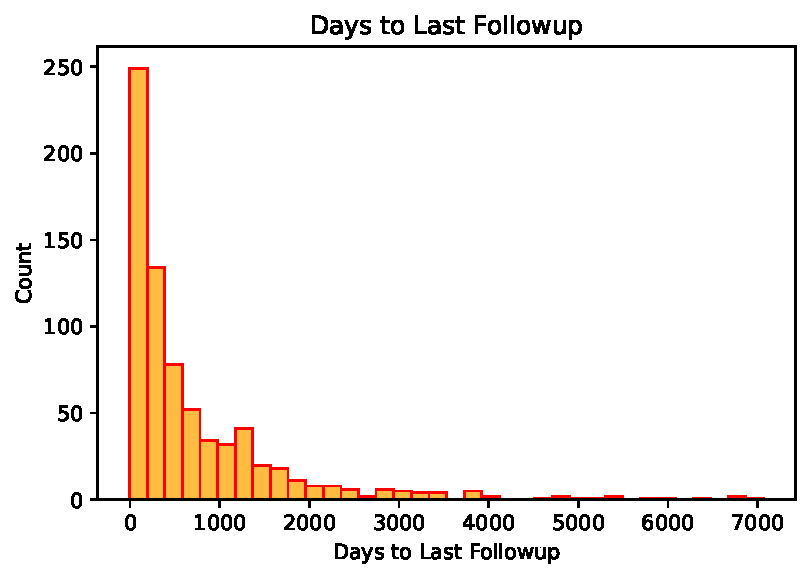
\includegraphics[width=.25\textwidth]{NOTEBOOK/IMAGENES_CRUDAS/18} 
			& 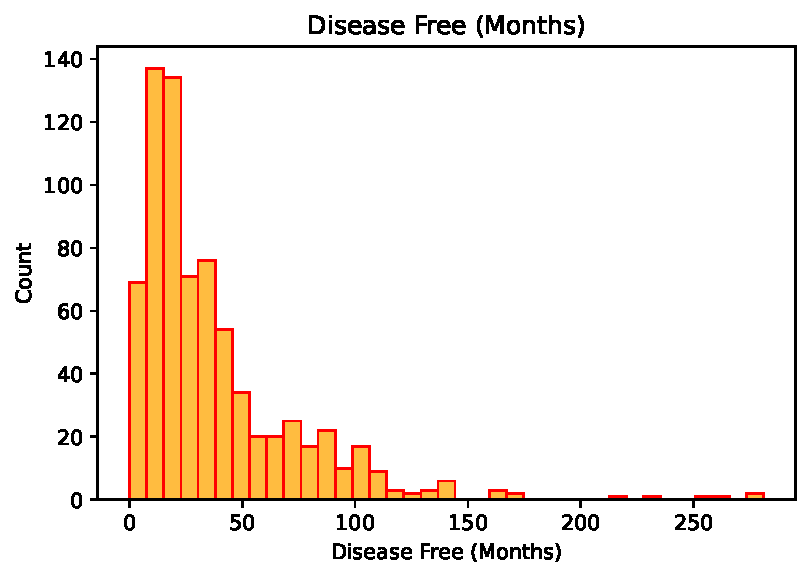
\includegraphics[width=.25\textwidth]{NOTEBOOK/IMAGENES_CRUDAS/19} 
			& 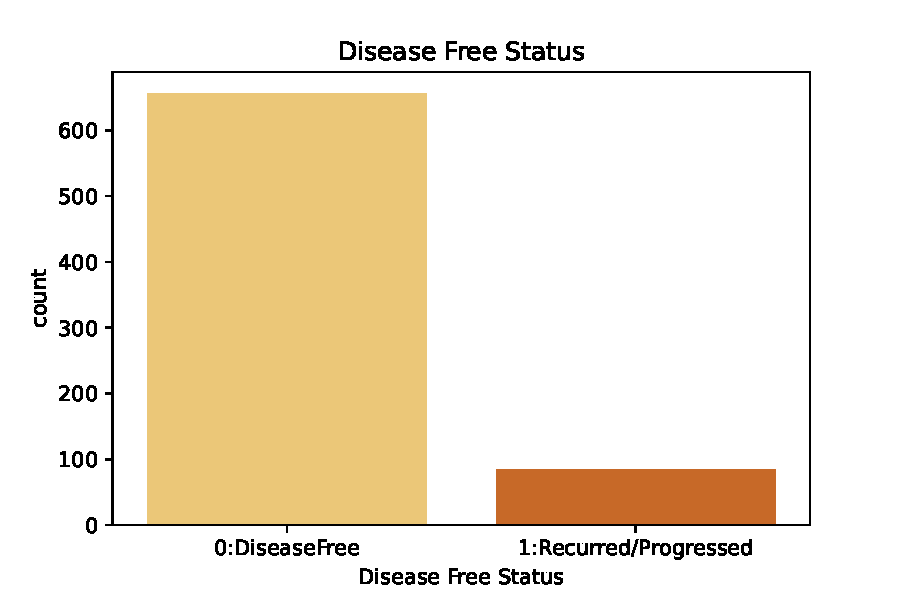
\includegraphics[width=.25\textwidth]{NOTEBOOK/IMAGENES_CRUDAS/20} 
			\\  \hline
			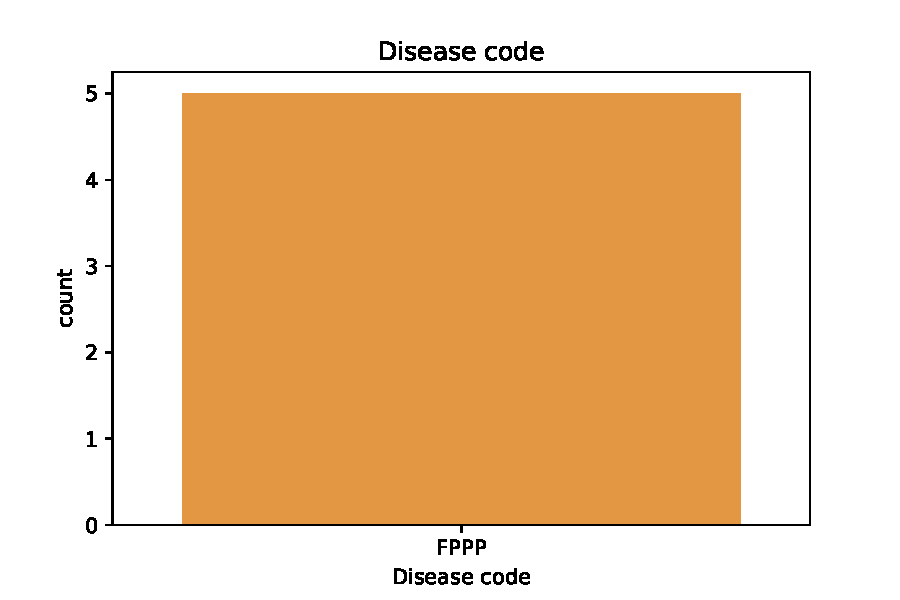
\includegraphics[width=.25\textwidth]{NOTEBOOK/IMAGENES_CRUDAS/21} 
			& 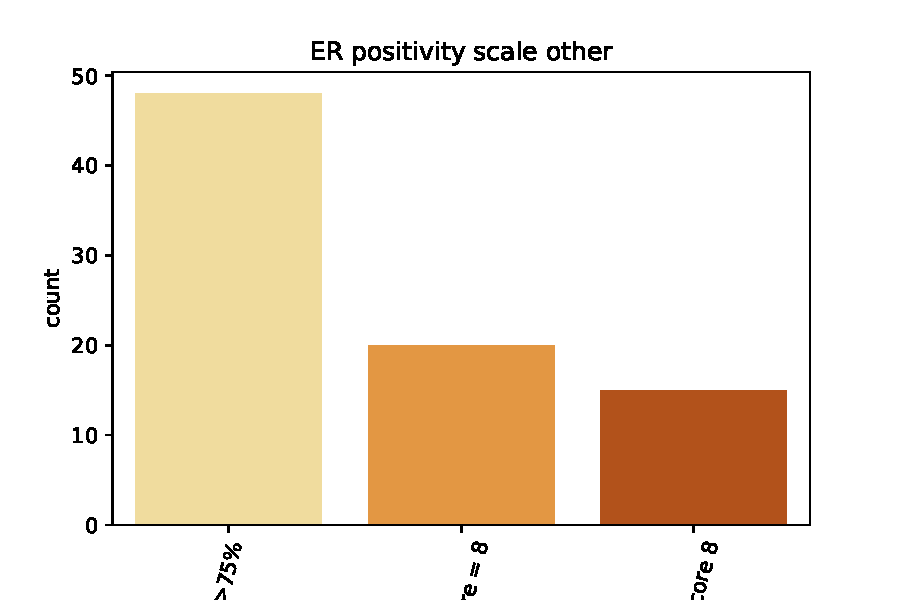
\includegraphics[width=.25\textwidth]{NOTEBOOK/IMAGENES_CRUDAS/22} 
			& 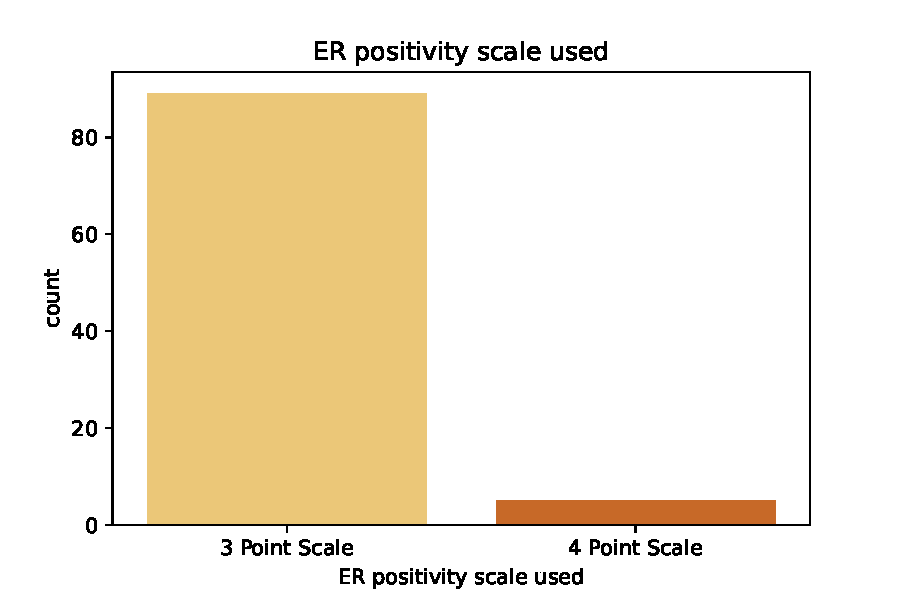
\includegraphics[width=.25\textwidth]{NOTEBOOK/IMAGENES_CRUDAS/23} 
			& 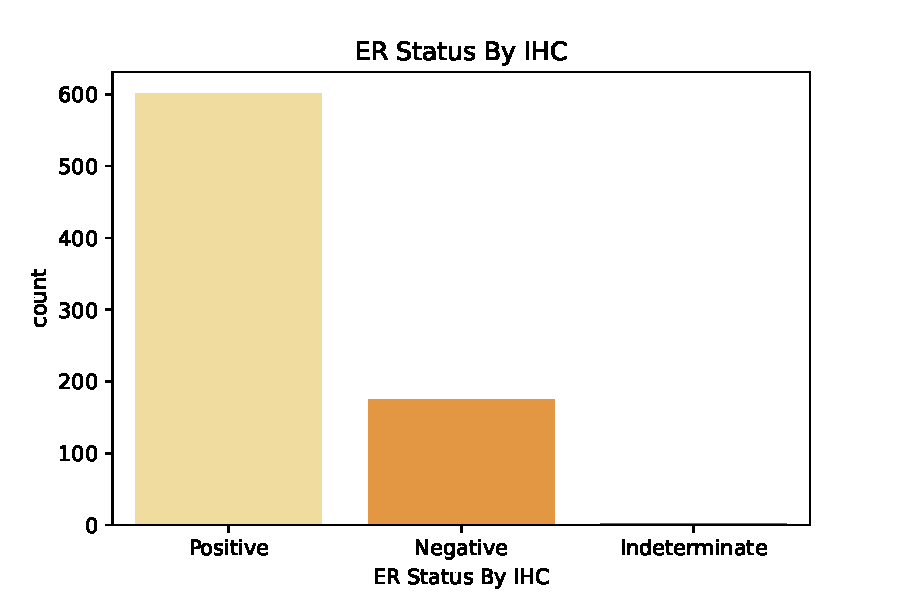
\includegraphics[width=.25\textwidth]{NOTEBOOK/IMAGENES_CRUDAS/24} 
			\\  \hline 
			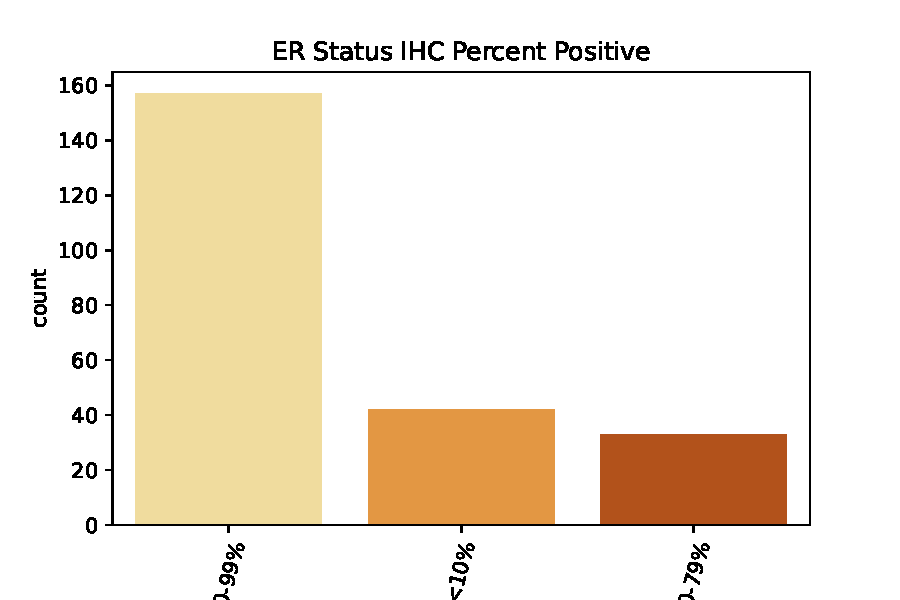
\includegraphics[width=.25\textwidth]{NOTEBOOK/IMAGENES_CRUDAS/25} 
			& 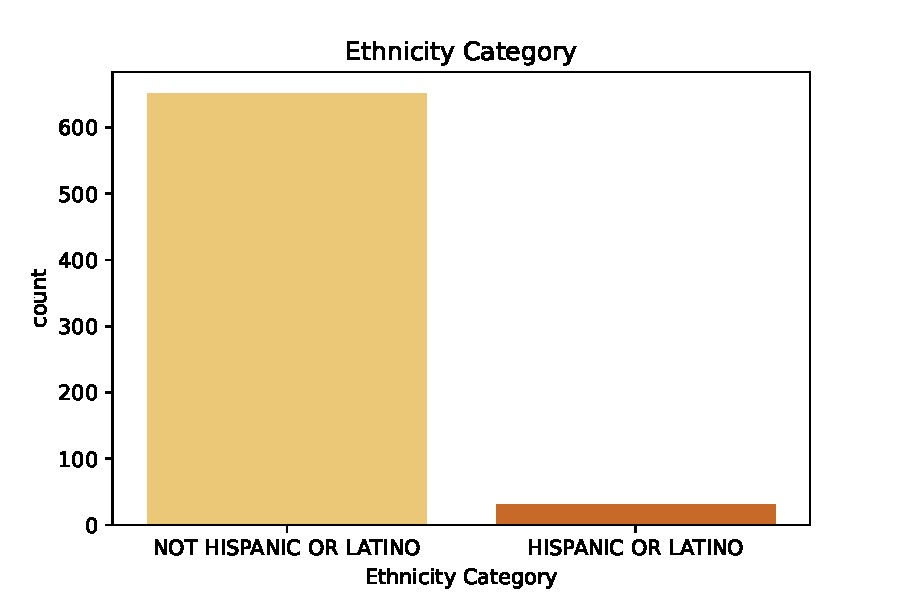
\includegraphics[width=.25\textwidth]{NOTEBOOK/IMAGENES_CRUDAS/26} 
			& 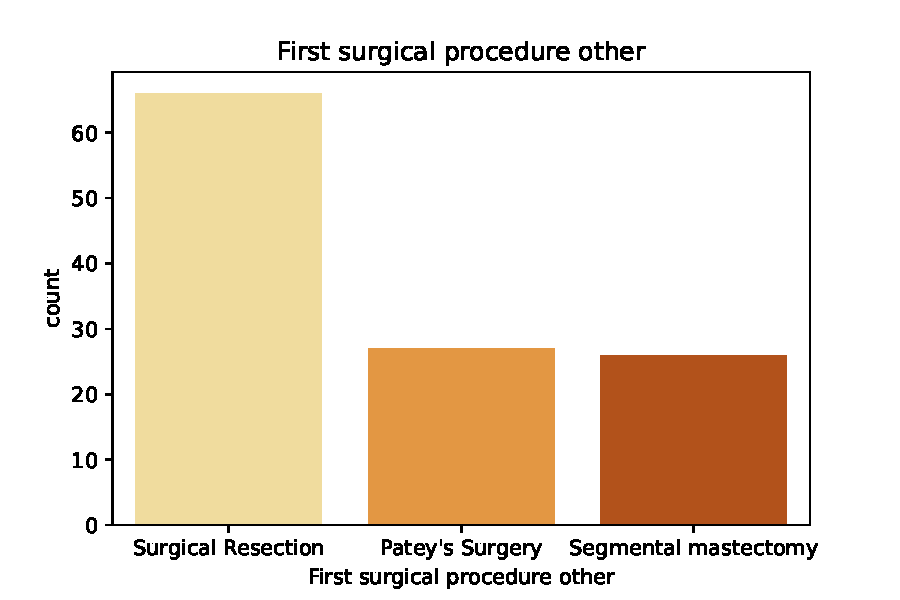
\includegraphics[width=.25\textwidth]{NOTEBOOK/IMAGENES_CRUDAS/27} 
			& 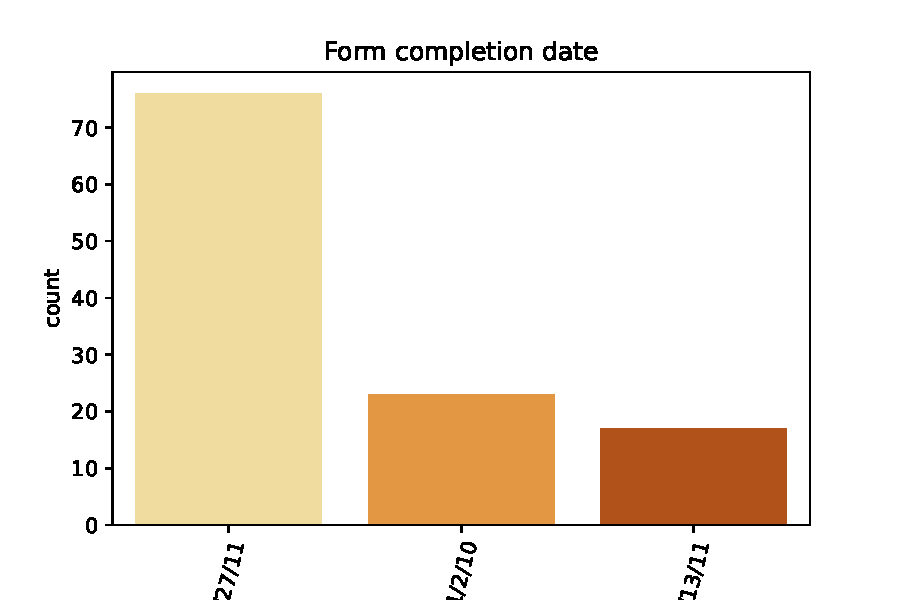
\includegraphics[width=.25\textwidth]{NOTEBOOK/IMAGENES_CRUDAS/28}   
			\\  \hline                
		\end{tabular} 
	\end{center} 
\end{table}

\clearpage
\begin{center} 
	\begin{tabular}{ |c|c|c|c| }  
		\hline 
		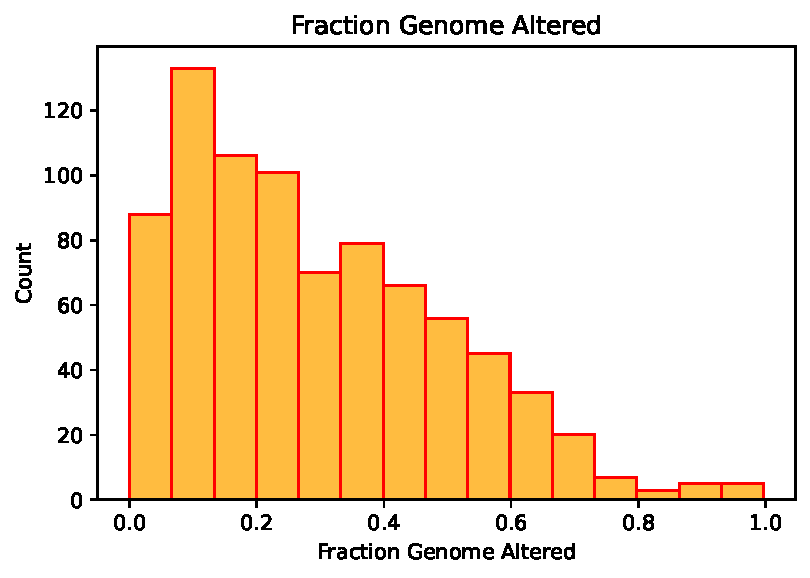
\includegraphics[width=.25\textwidth]{NOTEBOOK/IMAGENES_CRUDAS/29} 
		& 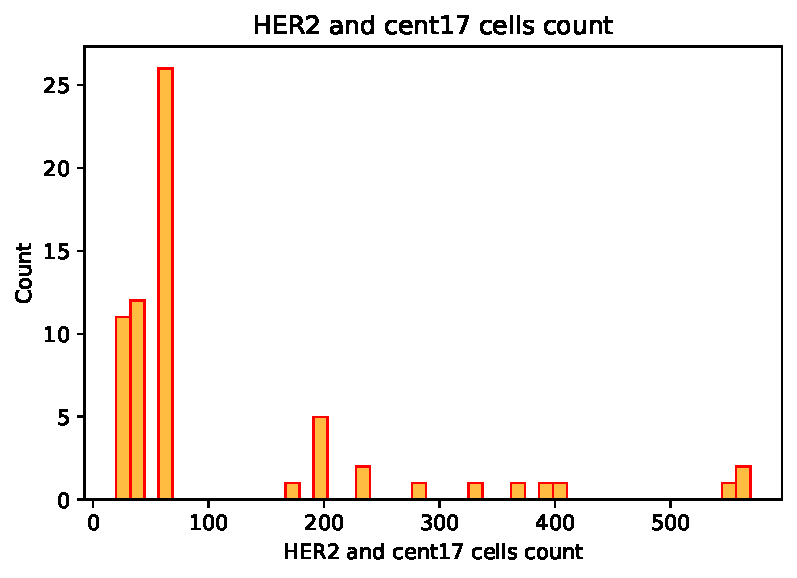
\includegraphics[width=.25\textwidth]{NOTEBOOK/IMAGENES_CRUDAS/30} 
		& 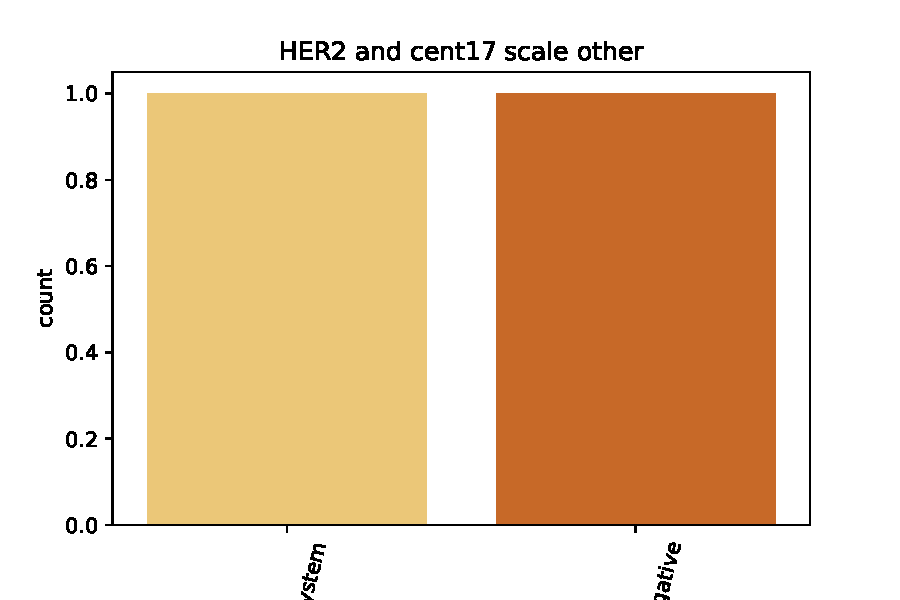
\includegraphics[width=.25\textwidth]{NOTEBOOK/IMAGENES_CRUDAS/31} 
		& 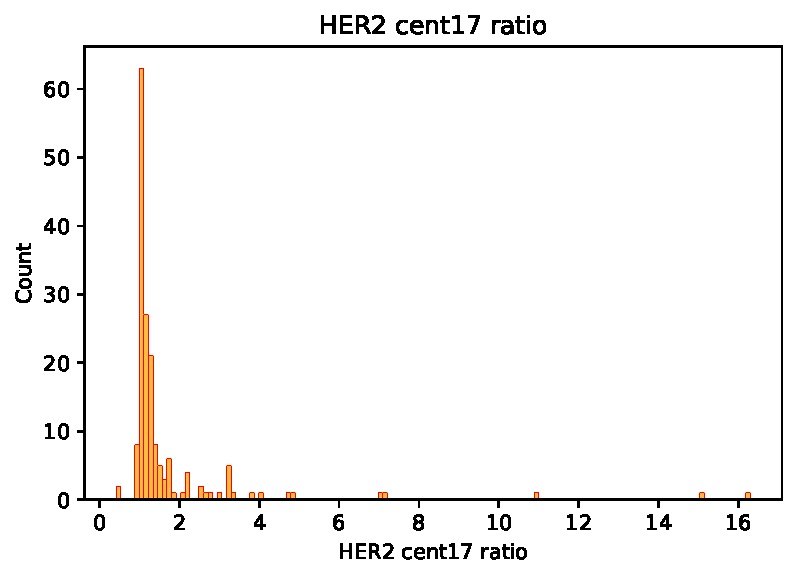
\includegraphics[width=.25\textwidth]{NOTEBOOK/IMAGENES_CRUDAS/32}   
		\\  \hline   
		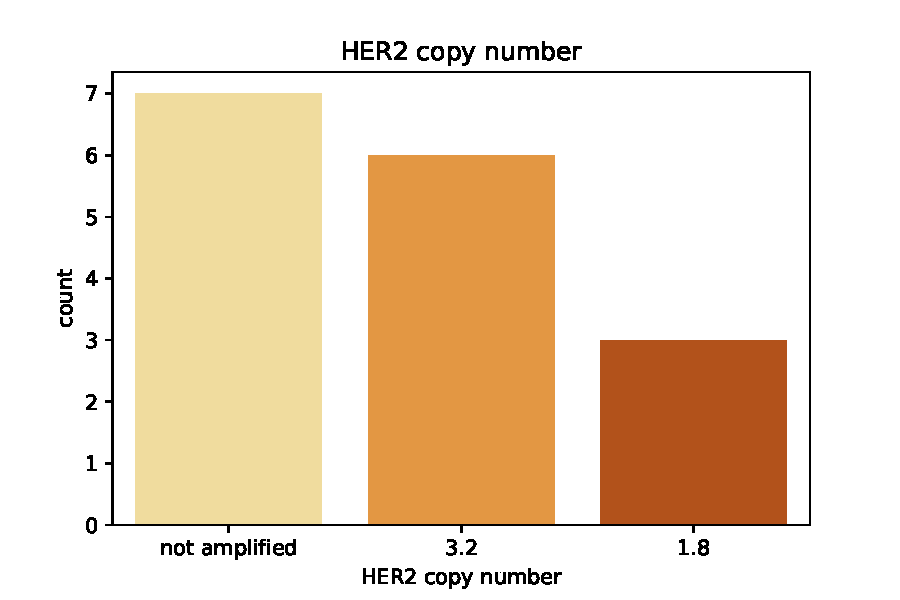
\includegraphics[width=.22\textwidth]{NOTEBOOK/IMAGENES_CRUDAS/33} 
		& 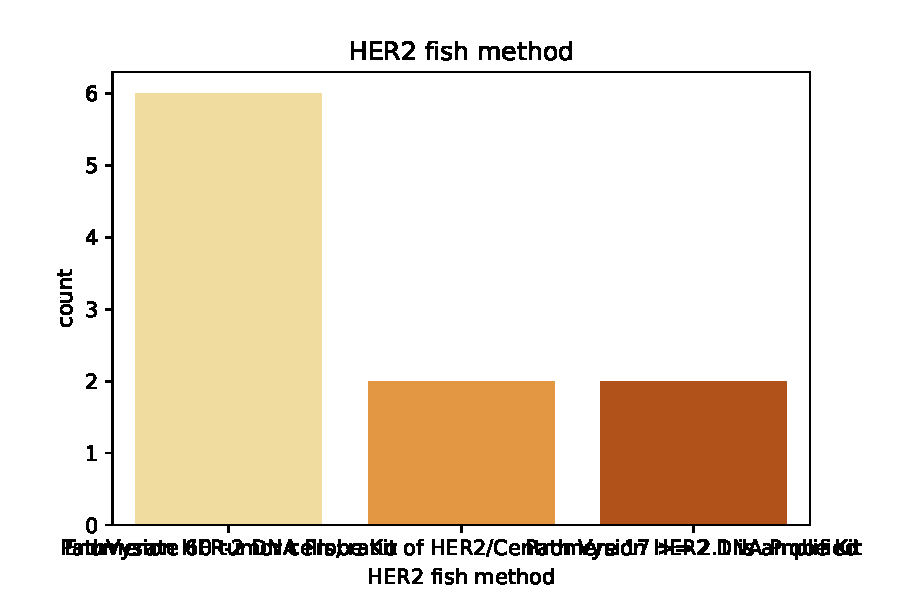
\includegraphics[width=.25\textwidth]{NOTEBOOK/IMAGENES_CRUDAS/34}
		& 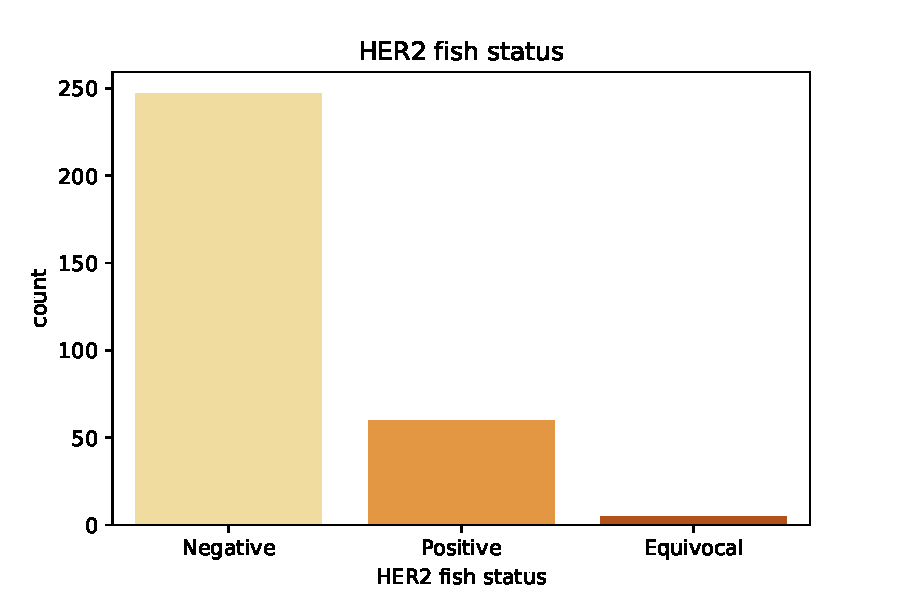
\includegraphics[width=.25\textwidth]{NOTEBOOK/IMAGENES_CRUDAS/35}
		& 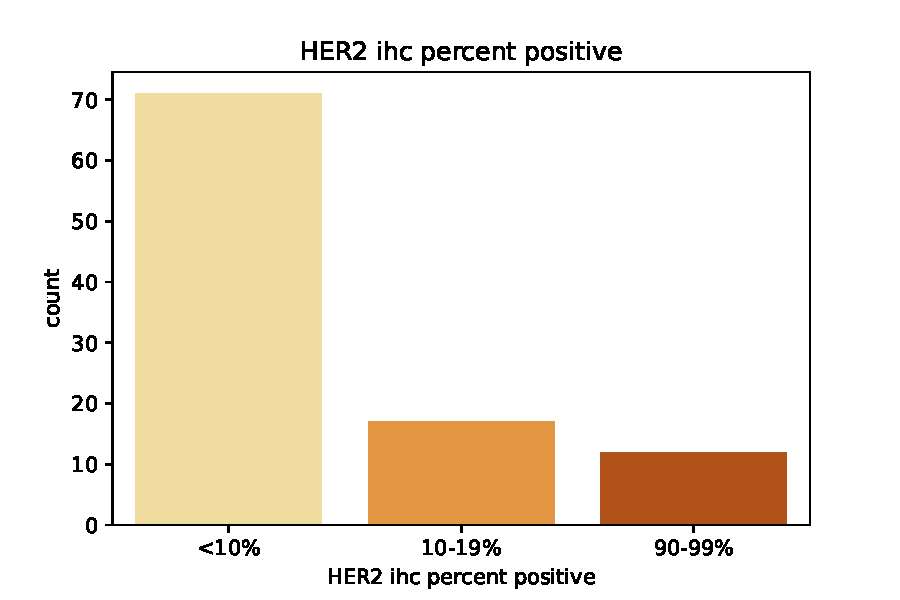
\includegraphics[width=.25\textwidth]{NOTEBOOK/IMAGENES_CRUDAS/36} 
		\\  \hline 
		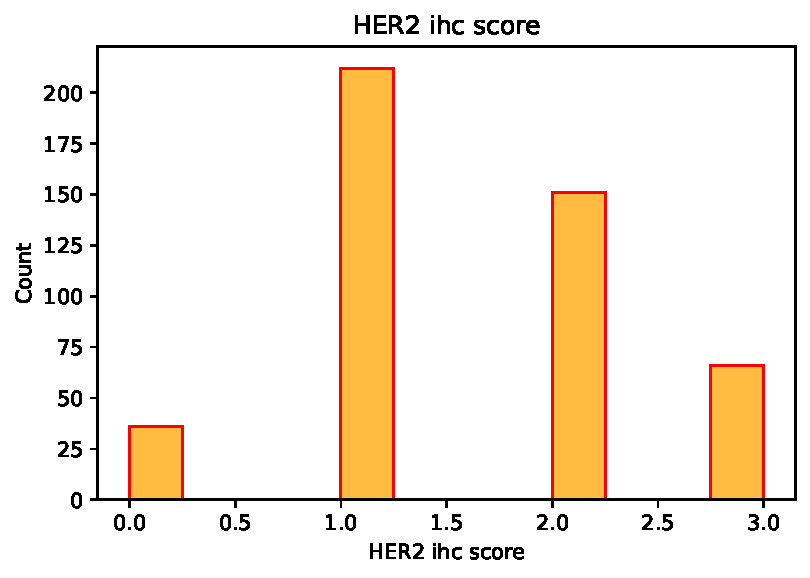
\includegraphics[width=.25\textwidth]{NOTEBOOK/IMAGENES_CRUDAS/37} 
		& 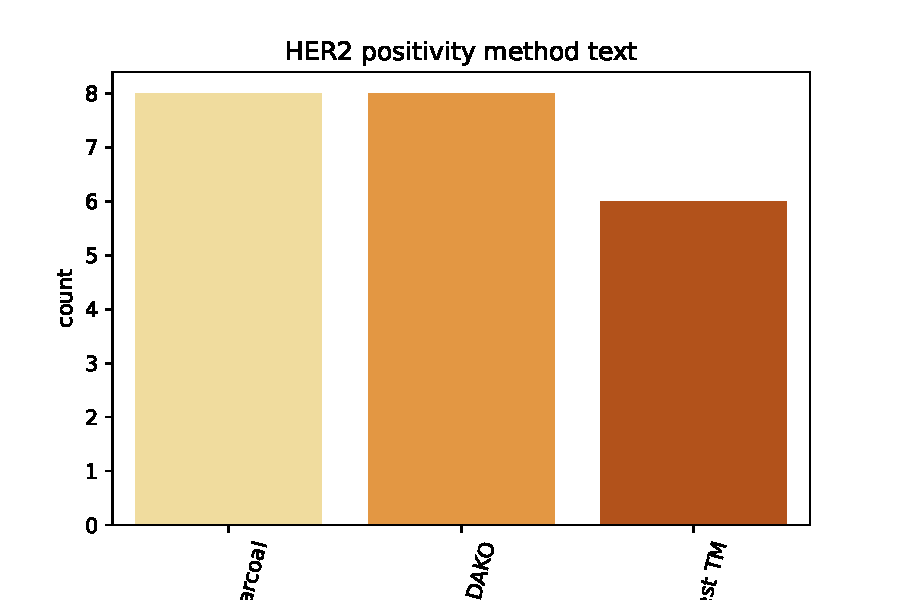
\includegraphics[width=.25\textwidth]{NOTEBOOK/IMAGENES_CRUDAS/38} 
		& 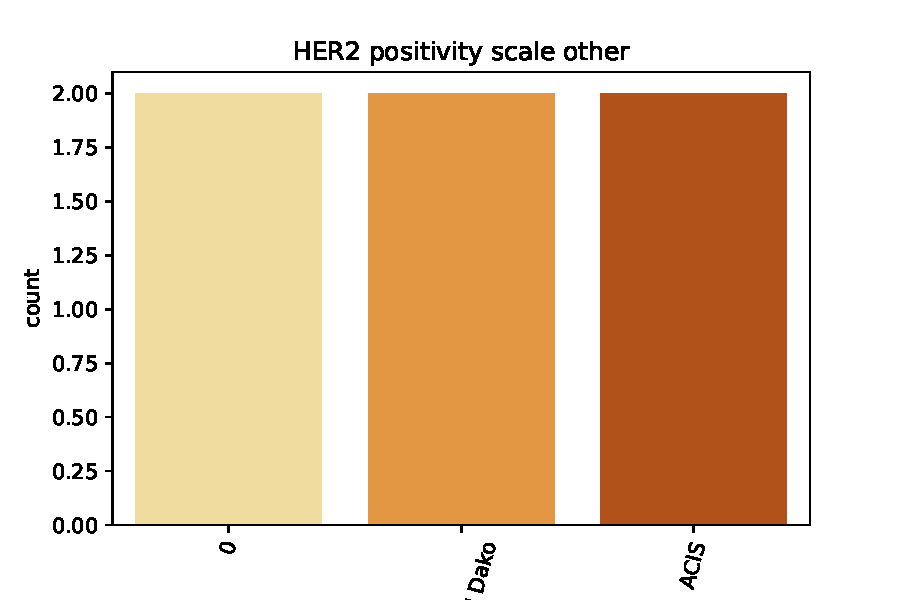
\includegraphics[width=.25\textwidth]{NOTEBOOK/IMAGENES_CRUDAS/39} 
		& 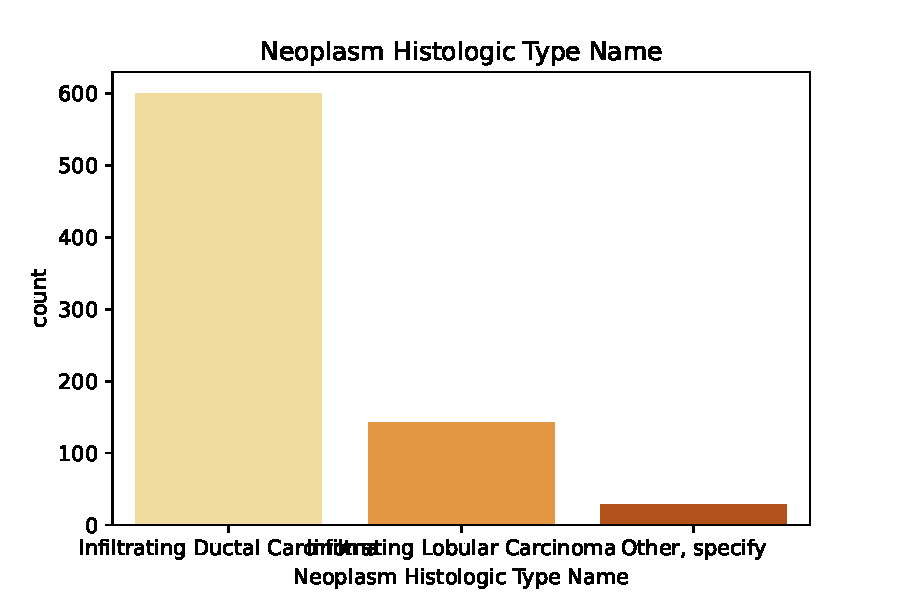
\includegraphics[width=.25\textwidth]{NOTEBOOK/IMAGENES_CRUDAS/40} 
		\\  \hline 
		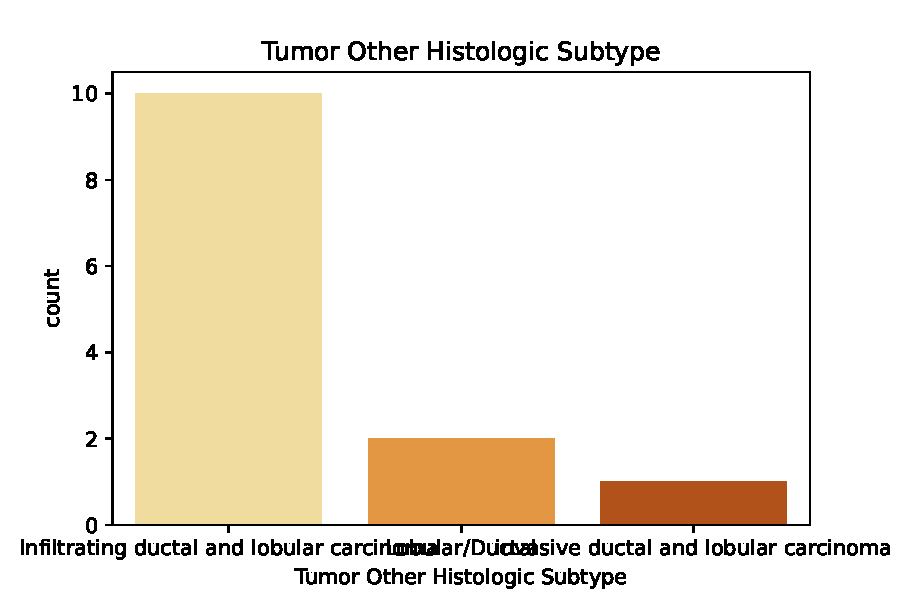
\includegraphics[width=.25\textwidth]{NOTEBOOK/IMAGENES_CRUDAS/41} 
		& 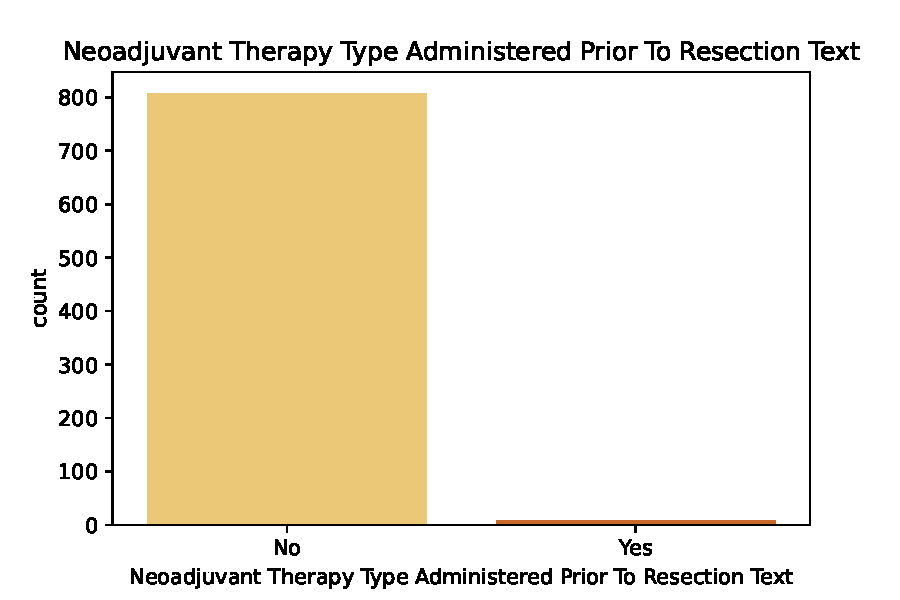
\includegraphics[width=.25\textwidth]{NOTEBOOK/IMAGENES_CRUDAS/42} 
		& 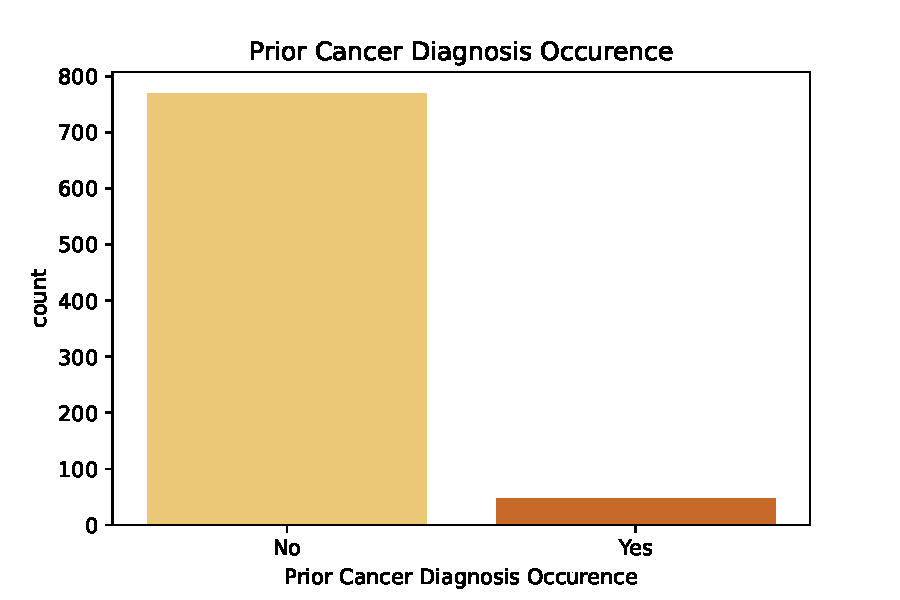
\includegraphics[width=.25\textwidth]{NOTEBOOK/IMAGENES_CRUDAS/43} 
		& 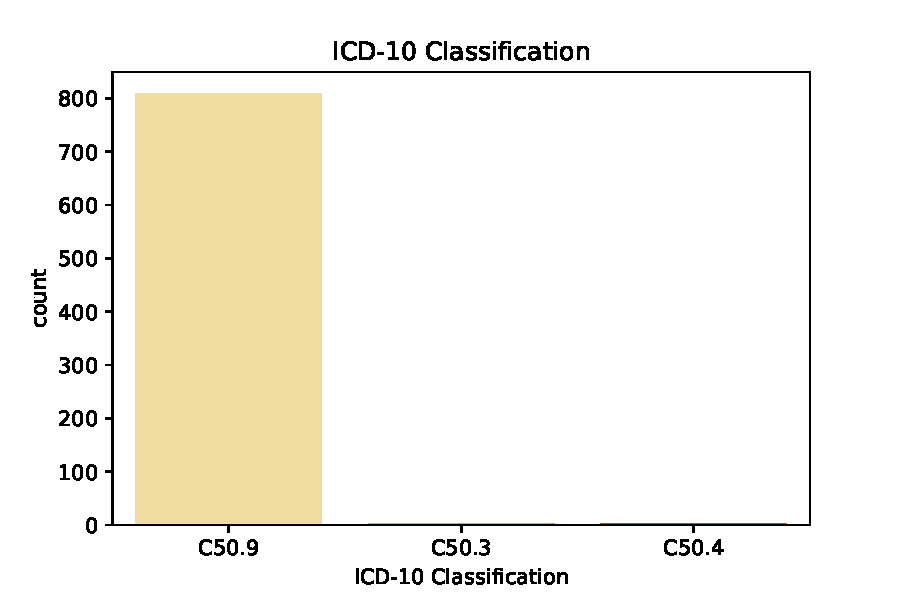
\includegraphics[width=.25\textwidth]{NOTEBOOK/IMAGENES_CRUDAS/44} 
		\\  \hline 
		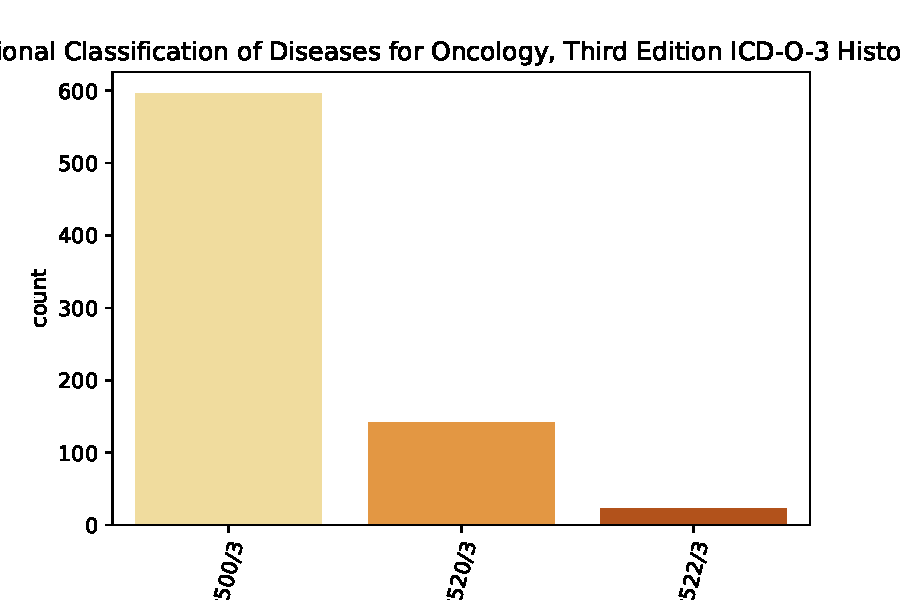
\includegraphics[width=.25\textwidth]{NOTEBOOK/IMAGENES_CRUDAS/45} 
		& 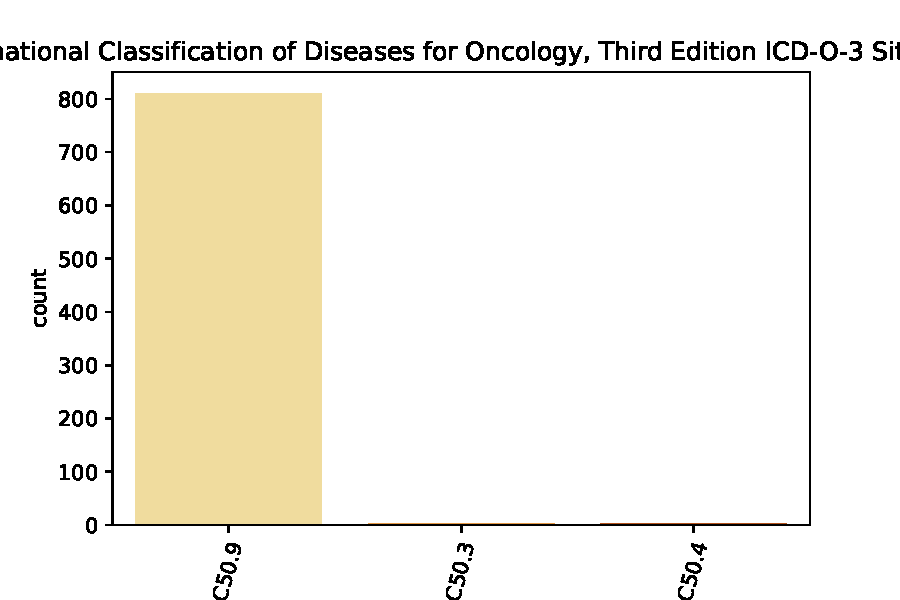
\includegraphics[width=.25\textwidth]{NOTEBOOK/IMAGENES_CRUDAS/46} 
		& 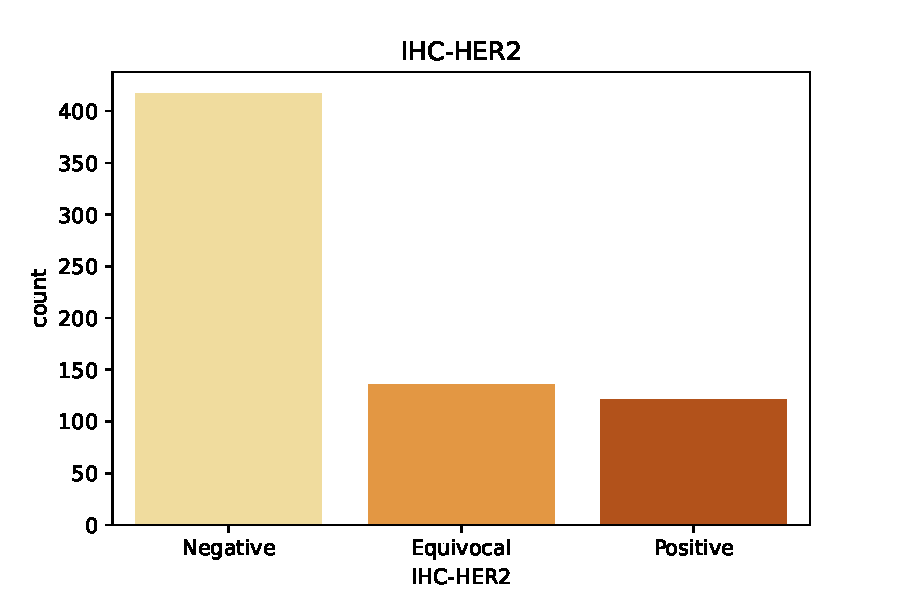
\includegraphics[width=.25\textwidth]{NOTEBOOK/IMAGENES_CRUDAS/47} 
		& 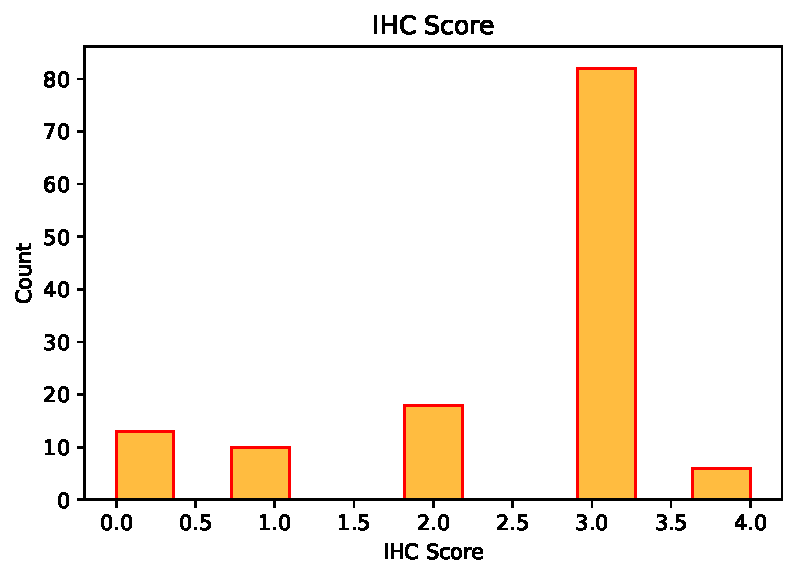
\includegraphics[width=.25\textwidth]{NOTEBOOK/IMAGENES_CRUDAS/48} 
		\\  \hline
		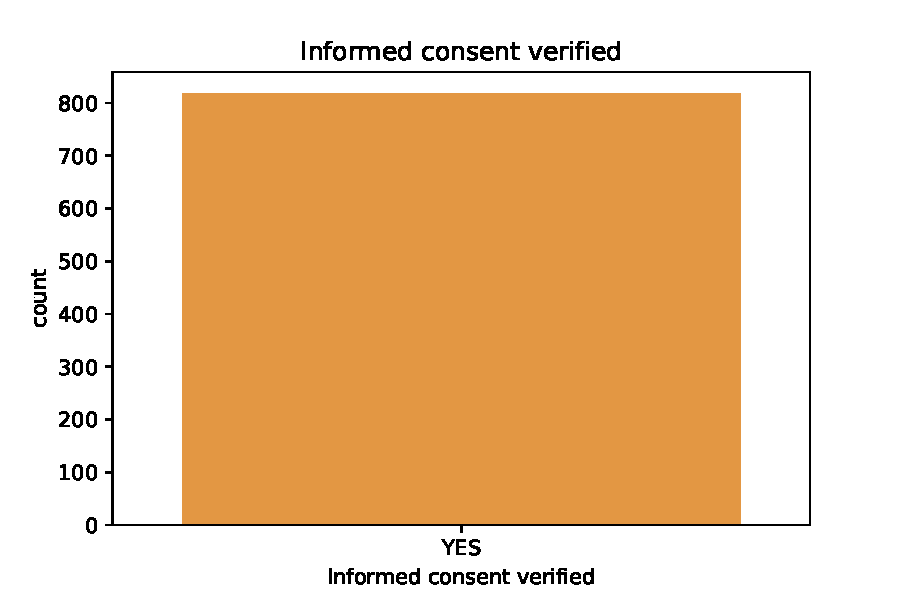
\includegraphics[width=.25\textwidth]{NOTEBOOK/IMAGENES_CRUDAS/49} 
		& 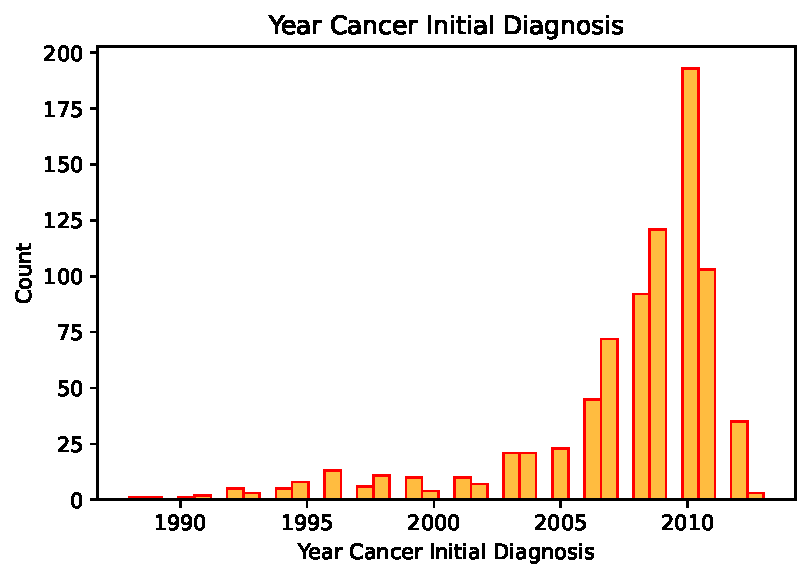
\includegraphics[width=.25\textwidth]{NOTEBOOK/IMAGENES_CRUDAS/50} 
		& \includegraphics[width=.25\textwidth]{NOTEBOOK/IMAGENES_CRUDAS/51} 
		& \includegraphics[width=.25\textwidth]{NOTEBOOK/IMAGENES_CRUDAS/52} 
		\\  \hline
		\includegraphics[width=.25\textwidth]{NOTEBOOK/IMAGENES_CRUDAS/53} 
		& \includegraphics[width=.25\textwidth]{NOTEBOOK/IMAGENES_CRUDAS/54} 
		& \includegraphics[width=.25\textwidth]{NOTEBOOK/IMAGENES_CRUDAS/55} 
		& \includegraphics[width=.25\textwidth]{NOTEBOOK/IMAGENES_CRUDAS/56} 
		\\  \hline         
	\end{tabular} 
\end{center} 

\begin{center} 
	\begin{tabular}{ |c|c|c|c| } 
		\hline 
		\includegraphics[width=.25\textwidth]{NOTEBOOK/IMAGENES_CRUDAS/57} 
		& \includegraphics[width=.25\textwidth]{NOTEBOOK/IMAGENES_CRUDAS/58} 
		& \includegraphics[width=.25\textwidth]{NOTEBOOK/IMAGENES_CRUDAS/59} 
		& \includegraphics[width=.25\textwidth]{NOTEBOOK/IMAGENES_CRUDAS/60}   
		\\  \hline       
		\hline 
		\includegraphics[width=.25\textwidth]{NOTEBOOK/IMAGENES_CRUDAS/61} 
		& \includegraphics[width=.25\textwidth]{NOTEBOOK/IMAGENES_CRUDAS/62} 
		& \includegraphics[width=.25\textwidth]{NOTEBOOK/IMAGENES_CRUDAS/63} 
		& \includegraphics[width=.25\textwidth]{NOTEBOOK/IMAGENES_CRUDAS/64}   
		\\  \hline    
		\includegraphics[width=.22\textwidth]{NOTEBOOK/IMAGENES_CRUDAS/65} 
		& \includegraphics[width=.25\textwidth]{NOTEBOOK/IMAGENES_CRUDAS/66}
		& \includegraphics[width=.25\textwidth]{NOTEBOOK/IMAGENES_CRUDAS/67}
		& \includegraphics[width=.25\textwidth]{NOTEBOOK/IMAGENES_CRUDAS/68} 
		\\  \hline 
		\includegraphics[width=.25\textwidth]{NOTEBOOK/IMAGENES_CRUDAS/69} 
		& \includegraphics[width=.25\textwidth]{NOTEBOOK/IMAGENES_CRUDAS/70} 
		& \includegraphics[width=.25\textwidth]{NOTEBOOK/IMAGENES_CRUDAS/71} 
		& \includegraphics[width=.25\textwidth]{NOTEBOOK/IMAGENES_CRUDAS/72} 
		\\  \hline 
		\includegraphics[width=.25\textwidth]{NOTEBOOK/IMAGENES_CRUDAS/73} 
		& \includegraphics[width=.25\textwidth]{NOTEBOOK/IMAGENES_CRUDAS/74} 
		& \includegraphics[width=.25\textwidth]{NOTEBOOK/IMAGENES_CRUDAS/75} 
		& \includegraphics[width=.25\textwidth]{NOTEBOOK/IMAGENES_CRUDAS/76} 
		\\  \hline 
		\includegraphics[width=.25\textwidth]{NOTEBOOK/IMAGENES_CRUDAS/77} 
		& \includegraphics[width=.25\textwidth]{NOTEBOOK/IMAGENES_CRUDAS/78} 
		& \includegraphics[width=.25\textwidth]{NOTEBOOK/IMAGENES_CRUDAS/79} 
		& \includegraphics[width=.25\textwidth]{NOTEBOOK/IMAGENES_CRUDAS/80} 
		\\  \hline
		\includegraphics[width=.25\textwidth]{NOTEBOOK/IMAGENES_CRUDAS/81} 
		& \includegraphics[width=.25\textwidth]{NOTEBOOK/IMAGENES_CRUDAS/82} 
		& \includegraphics[width=.25\textwidth]{NOTEBOOK/IMAGENES_CRUDAS/83} 
		& \includegraphics[width=.25\textwidth]{NOTEBOOK/IMAGENES_CRUDAS/84} 
		\\  \hline           
	\end{tabular} 
\end{center} 

\begin{center} 
	\begin{tabular}{ |c|c|c|c| }  
		\hline
		\includegraphics[width=.25\textwidth]{NOTEBOOK/IMAGENES_CRUDAS/85} 
		& \includegraphics[width=.25\textwidth]{NOTEBOOK/IMAGENES_CRUDAS/86} 
		& \includegraphics[width=.25\textwidth]{NOTEBOOK/IMAGENES_CRUDAS/87} 
		& \includegraphics[width=.25\textwidth]{NOTEBOOK/IMAGENES_CRUDAS/88} 
		\\  \hline 
		\includegraphics[width=.25\textwidth]{NOTEBOOK/IMAGENES_CRUDAS/89} 
		& \includegraphics[width=.25\textwidth]{NOTEBOOK/IMAGENES_CRUDAS/90} 
		& \includegraphics[width=.25\textwidth]{NOTEBOOK/IMAGENES_CRUDAS/91} 
		& \includegraphics[width=.25\textwidth]{NOTEBOOK/IMAGENES_CRUDAS/92}   
		\\  \hline    
		\includegraphics[width=.25\textwidth]{NOTEBOOK/IMAGENES_CRUDAS/93} 
		& \includegraphics[width=.25\textwidth]{NOTEBOOK/IMAGENES_CRUDAS/94} 
		& \includegraphics[width=.25\textwidth]{NOTEBOOK/IMAGENES_CRUDAS/95} 
		& \includegraphics[width=.25\textwidth]{NOTEBOOK/IMAGENES_CRUDAS/96}   
		\\  \hline     
		\includegraphics[width=.22\textwidth]{NOTEBOOK/IMAGENES_CRUDAS/97} 
		& \includegraphics[width=.25\textwidth]{NOTEBOOK/IMAGENES_CRUDAS/98}
		& \includegraphics[width=.25\textwidth]{NOTEBOOK/IMAGENES_CRUDAS/99}
		& \includegraphics[width=.25\textwidth]{NOTEBOOK/IMAGENES_CRUDAS/100} 
		\\  \hline 
		\includegraphics[width=.25\textwidth]{NOTEBOOK/IMAGENES_CRUDAS/101} 
		& \includegraphics[width=.25\textwidth]{NOTEBOOK/IMAGENES_CRUDAS/102} 
		& \includegraphics[width=.25\textwidth]{NOTEBOOK/IMAGENES_CRUDAS/103} 
		& \includegraphics[width=.25\textwidth]{NOTEBOOK/IMAGENES_CRUDAS/104} 
		\\  \hline 
		\includegraphics[width=.25\textwidth]{NOTEBOOK/IMAGENES_CRUDAS/105} 
		& \includegraphics[width=.25\textwidth]{NOTEBOOK/IMAGENES_CRUDAS/106} 
		& \includegraphics[width=.25\textwidth]{NOTEBOOK/IMAGENES_CRUDAS/107} 
		& \includegraphics[width=.25\textwidth]{NOTEBOOK/IMAGENES_CRUDAS/108} 
		\\  \hline                
	\end{tabular} 
	\begin{tabular}{ |c|c| }  
		\hline 
		\includegraphics[width=.22\textwidth]{NOTEBOOK/IMAGENES_CRUDAS/109} 
		& \includegraphics[width=.25\textwidth]{NOTEBOOK/IMAGENES_CRUDAS/110}
		\\  \hline 
	\end{tabular} 
\end{center} 

\newpage
\begin{figure}[!htb]
	\centering
	\includegraphics[width=1
	\linewidth]{NOTEBOOK/IMAGENES_PERDIDAS/missing_displot}
	\caption{Datos perdidos expresados en una gráfica de barras.}
	\label{Missing_Bar_Chart}
\end{figure}

 \begin{figure}[!htb]
	\centering
	\includegraphics[width=1
	\linewidth]{NOTEBOOK/IMAGENES_PERDIDAS/missing_heatmap}
	\caption{Datos perdidos expresados en un mapa espectral.}
	\label{Missing_Spectrum}
\end{figure}


\clearpage
En segundo lugar, basados en la obtención de los atributos del conjunto de datos \textit{“Breast Invasive Carcinoma (TCGA, Cell 2015)”}, se realizo un análisis de la cantidad de \textbf{datos ausentes} para identificar las variables y en la etapa posterior realizar la limpieza y el pre-procesamiento de los datos para hacerlos consistentes y sin ningún tipo de ruido. Los resultados obtenidos se pueden observar en el \textit{diagrama de barras} de la figura \ref{Missing_Bar_Chart}. 

Por ultimo con base a los resultados obtenidos en las gráficos unidimensionales  y  la identificación de datos ausentes, se realizo la validación con el experto en oncologia, en donde se tomo la decisión de eliminar \textit{69 variables} para realizar la fase de modelado y ejecución. Estas variables pueden ser observadas en la tabla \ref{data_no_relevante}. Lo anterior a causa de que no brindan informacion relevante para responder las preguntas planteadas en el \textit{BCQM}, la cantidad de datos no ERA suficiente para generar un análisis verídico o  no aportaban información de índole genético relacionada con los tipos de cáncer Lobulillar Invasivo (LBC), Ductal Invasivo (IDC) o de Tumores Mixtos (MTBC).

\begin{table*}[!htb]
	\footnotesize
	\centering
	\begin{threeparttable}
		\begin{tabular}{p{0.5cm} p{4cm} p{1.5cm} p{2cm} p{1.5cm} p{2cm} p{1.5cm}} \toprule
			$N$  &Variable &Distintas &Distintas($\%$) &Ausentes &Ausentes($\%$)  &Tamaño($kb$)
			%-----------------
			\\ \hline	1	&	Study ID	&	1	&	0,1	&	0	&	0	&	65,5
			\\ \hline	2	&	Patient ID	&	817	&	99,9	&	0	&	0	&	61,5
			\\ \hline	3	&	Sample ID	&	818	&	100	&	0	&	0	&	63,9
			\\ \hline	4	&	AJCC Version Type	&	5	&	0,7	&	97	&	11,9	&	47,9
			\\ \hline	5	&	Brachytherapy 	&	48	&	25,5	&	630	&	77	&	147
			\\ \hline	6	&	Cancer Type	&	1	&	0,1	&	0	&	0	&	71,9
			\\ \hline	7	&	Cent17 Copy Number	&	41	&	62,1	&	752	&	91,7	&	4,4
			\\ \hline	8	&	Birth nitial Diagnosis 	&	786	&	97,8	&	14	&	1,7	&	12,6
			\\ \hline	9	&	Days Sample Collection	&	584	&	71,6	&	2	&	0,2	&	12,8
			\\ \hline	11	&	Death Initial Diagnosis 	&	83	&	97,7	&	733	&	89,6	&	1,3
			\\ \hline	12	&	Alive Initial Diagnosis	&	1	&	0,1	&	1	&	0,1	&	54,3
			\\ \hline	10	&	Days to Last Followup	&	511	&	69,8	&	86	&	10,5	&	11,4
			\\ \hline	13	&	Disease code	&	1	&	20	&	813	&	99,4	&	0,345
			\\ \hline	14	&	ER positivity scale other	&	47	&	22,8	&	612	&	74,8	&	15,1
			\\ \hline	15	&	ER positivity scale used	&	2	&	2,1	&	724	&	88,5	&	7,2
			\\ \hline	16	&	First procedure other	&	61	&	26,6	&	589	&	72	&	20,2
			\\ \hline	17	&	Form completion date	&	234	&	28,6	&	0	&	0	&	57,4
			\\ \hline	18	&	HER2 and cent17 cells 	&	18	&	27,7	&	753	&	92	&	1
			\\ \hline	19	&	HER2 and cent17 scale 	&	2	&	100	&	816	&	98,9	&	0,182
			\\ \hline	20	&	HER2 cent17 ratio	&	63	&	37,3	&	649	&	79,3	&	2,6
			\\ \hline	21	&	HER2 copy number	&	50	&	67,6	&	744	&	91	&	5
			\\ \hline	22	&	HER2 fish method	&	18	&	66,7	&	791	&	96,7	&	2,6
			\\ \hline	23	&	HER2 positivity method 	&	12	&	31,6	&	780	&	85,3	&	3
			\\ \hline	24	&	HER2 positivity scale 	&	7	&	70	&	808	&	98	&	0,718
			\\ \hline	25	&	Tumor Histologic Subtype	&	13	&	56,6	&	795	&	97,2	&	2,2
			\\ \hline
		\end{tabular}
	\end{threeparttable}
\end{table*}
\clearpage
\begin{table*}[!htb]
	\footnotesize
	\centering
	\begin{threeparttable}
		\begin{tabular}{p{0.5cm} p{4cm} p{1.5cm} p{2cm} p{1.5cm} p{2cm} p{1.5cm}} \toprule
					26	&	Prior Cancer Diagnosis	&	2	&	0,2	&	1	&	0,1	&	53,5
		\\ \hline	27	&	ICD-10 Classification	&	7	&	0,9	&	0	&	0	&	55,9
		\\ \hline	28	&	ICD-O-3 Histology Code	&	17	&	2,1	&	0	&	0	&	56,7
		\\ \hline	29	&	ICD-O-3 Site Code	&	6	&	0,7	&	0	&	0	&	55,9
		\\ \hline	30	&	IHC Score	&	5	&	3,9	&	689	&	84,2	&	8,6
		\\ \hline	31	&	Informed consent verified	&	1	&	0,1	&	0	&	0	&	54,3
		\\ \hline	32	&	Is FFPE	&	1	&	0,1	&	0	&	0	&	54,3
		\\ \hline	33	&	Positive Lymph Keratin	&	5	&	2,1	&	579	&	70,8	&	15,9
		\\ \hline	34	&	Margin status reexcision	&	3	&	6,4	&	771	&	94,2	&	3,3
		\\ \hline	35	&	Metastatic Site	&	5	&	38,5	&	805	&	98,4	&	0,967
		\\ \hline	36	&	Metastatic Site Other	&	5	&	100	&	813	&	99,4	&	0,396
		\\ \hline	37	&	First Diagnosis Type	&	9	&	16,7	&	764	&	93,4	&	4,3
		\\ \hline	38	&	Neoplasm Event 	&	2	&	3,2	&	756	&	92,4	&	4,1
		\\ \hline	39	&	Nte cent 17 HER2 ratio	&	2	&	100	&	816	&	98,9	&	0,138
		\\ \hline	40	&	Nte er ihc intensity score	&	1	&	100	&	817	&	99,9	&	0,67
		\\ \hline	41	&	Nte er status	&	2	&	20	&	808	&	98,8	&	0,73
		\\ \hline	42	&	Nte er status ihc 	&	3	&	75	&	814	&	99,5	&	0,282
		\\ \hline	43	&	Nte HER2 fish status	&	1	&	33,3	&	815	&	99,6	&	0,219
		\\ \hline	44	&	Nte HER2 ihc score	&	2	&	66,7	&	815	&	99,6	&	0,201
		\\ \hline	45	&	Nte HER2 status	&	1	&	14,3	&	811	&	99,1	&	0,511
		\\ \hline	46	&	Nte HER2 status ihc 	&	1	&	50	&	816	&	99,8	&	0,138
		\\ \hline	47	&	Nte pr ihc intensity score	&	1	&	100	&	817	&	99,9	&	0,68
		\\ \hline	48	&	Nte pr status by ihc	&	2	&	22,2	&	809	&	98,9	&	0,657
		\\ \hline	49	&	Nte pr status ihc positive	&	1	&	50	&	816	&	99,8	&	0,138
		\\ \hline	50	&	Other Patient ID	&	817	&	99,9	&	0	&	0	&	80,7
		\\ \hline	51	&	Other Sample ID	&	817	&	100	&	1	&	0,1	&	80,6
		\\ \hline	52	&	Report File Name	&	817	&	100	&	1	&	0,1	&	94,1
		\\ \hline	53	&	Pharmaceutical Therapy 	&	2	&	3,8	&	766	&	93,6	&	3,4
		\\ \hline	54	&	Project code	&	1	&	20	&	813	&	99,4	&	0,345
		\\ \hline	55	&	PR positivity method	&	53	&	29,3	&	637	&	77,9	&	14,1
		\\ \hline	56	&	PR positivity ihc score	&	5	&	4,1	&	695	&	85,5	&	8
		\\ \hline	57	&	PR positivity scale other	&	47	&	25,3	&	632	&	77,3	&	13,7
		\\ \hline	58	&	PR positivity scale used	&	2	&	2,2	&	729	&	89,1	&	6,8
		\\ \hline	59	&	PR status ihc positive	&	10	&	3,5	&	529	&	64,7	&	19,9
		\\ \hline	60	&	adjuvant postoperative 	&	2	&	3,8	&	766	&	93,6	&	3,4
		\\ \hline	61	&	Tissue Retrospective 	&	2	&	0,2	&	1	&	0,1	&	54
		\\ \hline	62	&	Samples Per Patient	&	2	&	0,2	&	0	&	0	&	52,7
		\\ \hline	63	&	Sample Type	&	2	&	0,2	&	0	&	0	&	57,5
		\\ \hline	64	&	Somatic Status	&	1	&	0,1	&	0	&	0	&	57,5
		\\ \hline	65	&	Staging System 1	&	16	&	94,1	&	801	&	97,9	&	1,7
		\\ \hline	66	&	Surgery margins	&	4	&	10	&	778	&	95,1	&	3,1
		\\ \hline	67	&	Surgery margins other	&	11	&	100	&	807	&	98,7	&	0,977
		\\ \hline	68	&	Tissue Source Site	&	24	&	2,9	&	1	&	0,1	&	53,5
		\\ \hline	69	&	Tumor Anatomic Site	&	1	&	0,1	&	1	&	0,1	&	56,6
		\\ \hline
		\end{tabular}
		\caption{Estadísticas de variables no relevantes.}
		\label{data_no_relevante}
	\end{threeparttable}
\end{table*}
\clearpage
\newpage
\subsection{Transformación de variables genómicas}
En este parte del análisis exploratorio de datos oncológicos, se procesaron las variables por medio de algoritmos en \textit{Python} para que la información quedara estandarizada y así garantizar que los resultados generados por los modelos de ML fueran consistentes y veraces. Cabe resaltar, que aunque en la fase anterior se detectaron las variables que por su falta de datos o poco aporte en el análisis requerido tuvieron que ser eliminadas, en esta fase aun así se reajustaron para garantizar que no se presentara un falso positivo por falta de estandarización y así garantizar que no se eliminara una variable por equivocación.

\subsubsection{Renombramiento de columnas}
En esta parte de la transformación de datos, se renombraron los nombres de las variables, ya que como observamos anteriormente presentaban una longitud extensa. Esto se realizó con el propósito de garantizar el desempeño de los modelos de ML. Para lograrlo, se utilizó la función $clean\_headers()$ de la librería \textit{dataprep.eda}, lo cual permitió limpiar los encabezados y estandarizarlos en el formato \textit{snake} que tiene la estructura \textit{“nombre\_columna”}. En el algoritmo \ref{renombramiento} se puede observar el código implementado.

\begin{lstlisting}[basicstyle=\scriptsize,language=Python, label=renombramiento, caption=Renombramiento de columnas en Python.]
	# Importar librerias
	import pandas as pd
	import numpy as np
	from dataprep.clean import clean_headers
	
	# Abrir conjunto de datos delimitados por espacios
	with open('brca_tcga_pub2015_clinical_data.csv') as f:
	breast_cancer=pd.read_csv(f, delimiter="\t")
	
	# Generar una copia del data-set original
	bc = breast_cancer.copy()
	bc.shape
	
	# Estandarizar cabecera en format snake
	bc=clean_headers(breast_cancer)
	
	# Reemplazar nomenclatura extensa
	bc.columns=bc.columns.str.replace('american_joint_committee_on_cancer_','')
	bc.columns=bc.columns.str.replace('international_classification_of_diseases_for_oncology_third_edition_icd_o_3_','')
	
	# Renombrar variables con un nombre corto
	bc.rename(
	columns={
		'neoplasm_disease_lymph_node_stage_code':'neoplasm_lymph_code',
		'neoplasm_lymph_node_stage_code':'neoplasm_stage',
		'brachytherapy_first_reference_point_administered_total_dose':'brachytherapy',
		'birth_from_initial_pathologic_diagnosis_date':'birth_initial_diagnosis',
		'death_from_initial_pathologic_diagnosis_date':'death_initial_diagnosis',
		'last_alive_less_initial_pathologic_diagnosis_date_calculated_day_value':'last_alive_date',
		'neoadjuvant_therapy_type_administered_prior_to_resection_text':'neoadjuvant_therapy',
		'prior_cancer_diagnosis_occurence':'prior_diagnosis_occurence',
		'informed_consent_verified':'consent_verified',
		'primary_lymph_node_presentation_assessment_ind_3':'lymph_presentation',
		'positive_finding_lymph_node_hematoxylin_and_eosin_staining_microscopy_count':'positive_lymph_hematoxylin',
		'positive_finding_lymph_node_keratin_immunohistochemistry_staining_method_count':'positive_lymph_keratin',
		'lymph_node_s_examined_number':'lymph_examined_number',
		'first_pathologic_diagnosis_biospecimen_acquisition_method_type':'biospecimen_method',
		'first_pathologic_diagnosis_biospecimen_acquisition_other_method_type':'biospecimen_other_method',
		'new_neoplasm_event_post_initial_therapy_indicator':'new_neoplasm_event',
		'adjuvant_postoperative_pharmaceutical_therapy_administered_indicator':'pharmaceutical_therapy',
		'tissue_prospective_collection_indicator':'tissue_prospective_indicator',
		'did_patient_start_adjuvant_postoperative_radiotherapy':'postoperative_radiotherapy',
		'tissue_retrospective_collection_indicator':'tissue_retrospective_indicator',
		'number_of_samples_per_patient':'number_samples',
		'surgery_for_positive_margins':'surgery_positive',
		'surgery_for_positive_margins_other':'surgery_positive_other',
		'surgery_for_positive_margins_other':'surgery_positive_other',
		'neoplasm_histologic_type_name':'neoplasm_histologic_type',
		'tumor_other_histologic_subtype':'tumor_other_subtype',
		'year_cancer_initial_diagnosis':'year_initial_diagnosis',
		'first_surgical_procedure_other':'surgical_other'
	}, inplace=True)
	
	# Reemplazar artículos, pronombres y preposiciones
	bc.columns=bc.columns.str.replace('_to_','_')
	bc.columns=bc.columns.str.replace('_and_','_')
	bc.columns=bc.columns.str.replace('_by_','_')
	
\end{lstlisting}

\subsubsection{Estandarización de datos genómicos}
En esta parte de la transformación de datos, se estandarizaron los registros de cada columna para que quedaran en \textit{minúscula}. Para lograrlo, se utilizó la función $clean\_text()$ de la librería \textit{dataprep.eda}. Adicionalmente, se identificaron las variables que son \textit{únicas} y se homogeneizaron para que los datos quedaran uniformes. En el algoritmo \ref{estandarizacion} se puede observar el código implementado.

\begin{lstlisting}[basicstyle=\scriptsize,language=Python, label=estandarizacion, caption=Estandarización de datos genómicos en Python.]
	# Procesar datos para que queden en minuscula
	custom_pipeline = [{"operator": "lowercase"}]
	for i in bc.columns:
	bc=clean_text(bc,i,pipeline=custom_pipeline)
	
	# Estandarizar variables tipo NaN
	bc=bc.replace(
	["<NA>",
	"nan",
	"nan"
	],[np.NaN,
	np.NaN,
	np.NaN
	],regex=True)
	
	# Estandarizar variable brachytherapy
	bc.brachytherapy=bc.brachytherapy.replace(
	['no value given',
	'% ihc',
	'-',
	' '],
	[np.NaN,
	'ihc',
	'',
	''],regex=True)
	
	# Estandarizar variable publication_version_type
	bc.publication_version_type=bc.publication_version_type.replace(
	['th|rd'],[''],regex=True)
	
	# Estandarizar variable cent_17_copy_number
	bc.cent_17_copy_number=bc.cent_17_copy_number.replace(
	['polisomy',],[np.NaN,],regex=True)
	
	# Estandarizar variable er_positivity_scale_used
	bc.er_positivity_scale_used=bc.er_positivity_scale_used.replace(
	['point scale',],
	[''],regex=True)
	
	# Estandarizar variable disease_free_status
	bc.disease_free_status=bc.disease_free_status.replace(
	['0:diseasefree',
	'1:recurred/progressed'],
	['diseasefree',
	'progressed'],regex=True)
	
	# Estandarizar variable days_last_followup
	bc.days_last_followup = bc.days_last_followup.replace(
	['-'],[''],regex=True)
	
	
	# Estandarizar variable her_2_copy_number
	bc.her_2_copy_number=bc.her_2_copy_number.replace(
	['<',
	'>',
	'not amplified'
	],
	['',
	'',
	0],regex=True)
	
	# Estandarizar variable er_positivity_scale_other
	bc.er_positivity_scale_other=bc.er_positivity_scale_other.replace(
	['protein',
	'allred score 0',
	'=',
	'scrore',
	'h-score',
	'intensity',
	'strong using weak, moderate and strong',
	'moderate using the scale of weak, moderate, strong',
	'moderate using scale of weak, moderate, strong',
	' \(per outside facility\)',
	'  ',
	' '
	],
	['',
	'allred score',
	'',
	'score',
	'hscore',
	'',
	'strong',
	'moderate',
	'moderate',
	'',
	'',
	''
	],regex=True)
	
	# Estandarizar variable er_status_ihc
	bc.er_status_ihc=bc.er_status_ihc.replace(
	['indeterminate'],
	['positive'],regex=True)
	
	# Estandarizar variable er_status_ihc
	bc.er_status_ihc=bc.er_status_ihc.replace(
	['indeterminate'],
	['positive'],regex=True)
	
	# Estandarizar variable her_2_fish_status
	bc.her_2_fish_status=bc.her_2_fish_status.replace(
	['equivocal',
	'indeterminate'],
	['negative',
	'negative'],regex=True)
	
	# Estandarizar variable neoplasm_histologic_type
	bc.neoplasm_histologic_type=bc.neoplasm_histologic_type.replace(
	["(please specify)",
	"other, specify",
	'\(','\)'],
	['',
	'other',
	'',''],regex=True)
	
	# Estandarizar variable menopause_status
	bc.menopause_status=bc.menopause_status.replace(
	['post \(prior bilateral ovariectomy or >12 mo since lmp with no prior hysterectomy\)',
	'pre \(<6 months since lmp and no prior bilateral ovariectomy and not on estrogen replacement\)',
	'indeterminate \(neither pre or postmenopausal\)',
	'peri \(6-12 months since last menstrual period\)'
	],
	['post',
	'pre',
	'peri',
	'peri'],regex=True)
	
	# Estandarizar variable metastatic_site
	bc.metastatic_site=bc.metastatic_site.replace(
	['lung\|bone\|liver\|other, specify',
	'other, specify',
	'bone\|liver',
	],
	['other',
	'other',
	'bone-liver',],regex=True)
	
	# Estandarizar variable biospecimen_method
	bc.biospecimen_method=bc.biospecimen_method.replace(
	['other method, specify:',
	'cytology \(e.g. peritoneal or pleural fluid\)'
	],
	['other',
	'cytology'
	],regex=True)
	
	# Estandarizar variable biospecimen_method
	bc.biospecimen_method=bc.biospecimen_method.replace(
	['other method, specify:',
	'cytology \(e.g. peritoneal or pleural fluid\)'
	],
	['other',
	'cytology'
	],regex=True)
	
	# Estandarizar variable overall_survival_status
	bc.overall_survival_status=bc.overall_survival_status.replace(
	['0:',
	'1:'],
	['',
	''],regex=True)
	
	# Estandarizar variable tissue_prospective_indicator
	bc.tissue_prospective_indicator=bc.tissue_prospective_indicator.replace(
	['yes',
	'no'],
	['prospective',
	'retrospective'],regex=True)
	
	# Estandarizar variable pr_positivity_define_method
	bc.pr_positivity_define_method=bc.pr_positivity_define_method.replace(
	['no value given',
	'%ihc',
	'per outside facility report',
	'-',
	' ',
	],[np.NaN,
	'ihc',
	'',
	'',
	''],regex=True)
	
	# Estandarizar variable pr_positivity_scale_other
	bc.pr_positivity_scale_other=bc.pr_positivity_scale_other.replace(
	['protein',
	'allred score 0',
	'=',
	'scrore',
	'h-score',
	'intensity',
	'strong using weak, moderate and strong',
	'moderate using the scale of weak, moderate, strong',
	'moderate using scale of weak, moderate, strong',
	' \(per outside facility\)',
	'per outside facility report',
	'strong, using scale of weak, moderate and strong',
	'allread',
	'  ',
	' ',
	],
	['',
	'allred score',
	'',
	'score',
	'hscore',
	'',
	'strong',
	'moderate',
	'moderate',
	'',
	'',
	'Strong',
	'allred',
	'',
	'',
	],regex=True)
	
	# Estandarizar variable staging_system
	bc.staging_system=bc.staging_system.replace(
	['other \(specify\)'
	],
	['other'
	],regex=True)
	
	# Estandarizar variable staging_system_1
	bc.staging_system_1=bc.staging_system_1.replace(
	['sln and non-sln bx|'+
	'sln and non-sln biopsy|'+
	'sentinel ln and one non sentinel ln|'
	'sentinel \+ non sentinel|'
	'sn\+1 non sentinel node|'
	'sentinel lymph node biopsy and non-sentinel lymph node biopsy'
	],
	['sentinel lymph node and non-sentinel lymph node biopsy'
	],regex=True)
	
	# Estandarizar variable pr_positivity_ihc_intensity_score
	bc.pr_positivity_ihc_intensity_score=bc.pr_positivity_ihc_intensity_score.replace(
	['\+'],[''],regex=True)
	
	# Estandarizar variable pr_positivity_scale_used
	bc.pr_positivity_scale_used=bc.pr_positivity_scale_used.replace(
	['point scale',],
	[''],regex=True)
	
	# Estandarizar variable pr_status_ihc
	bc.pr_status_ihc=bc.pr_status_ihc.replace(
	['indeterminate'],
	['positive'],regex=True)
	
	# Estandarizar variable primary_tumor_site
	bc.primary_tumor_site=bc.primary_tumor_site.replace(
	['left',
	'left upper outer quadrant',
	'left upper inner quadrant',
	'right',
	'right upper outer quadrant',
	'right upper outer quadrant|right',
	'right lower outer quadrant|right',
	'right lower outer quadrant',
	'left lower outer quadrant',
	'right upper inner quadrant',
	'right lower inner quadrant',
	'left upper inner quadrant|left upper outer quadrant|left lower inner quadrant|left lower outer quadrant',
	'left upper inner quadrant|left upper outer quadrant',
	'right|right upper outer quadrant',
	'left upper outer quadrant|left',
	'left lower inner quadrant',
	'right upper inner quadrant|right lower inner quadrant',
	'left upper outer quadrant|left lower outer quadrant',
	'left upper outer quadrant|left lower outer quadrant|left',
	'left lower inner quadrant|left lower outer quadrant|left',
	'right upper inner quadrant|right upper outer quadrant',
	'right lower inner quadrant|right lower outer quadrant',
	'right upper outer quadrant|right lower outer quadrant',
	'left lower outer quadrant|left',
	'right upper inner quadrant|right',
	'left lower inner quadrant|left',
	'left upper inner quadrant|left upper outer quadrant|left',
	'right upper inner quadrant|right upper outer quadrant|right',
	'right lower inner quadrant|right lower outer quadrant|right',
	'left upper inner quadrant|left upper outer quadrant|left lower inner quadrant|left lower outer quadrant|left',
	'right upper inner quadrant|right lower inner quadrant|right',
	'left upper inner quadrant|left lower inner quadrant|left lower outer quadrant|left',
	'right upper inner quadrant|right upper outer quadrant|right lower inner quadrant|right lower outer quadrant|right',
	'left upper inner quadrant|left',
	'right upper outer quadrant|right lower inner quadrant|right lower outer quadrant',
	'right|right upper inner quadrant',
	'left upper inner quadrant|left lower inner quadrant',
	'left|left upper outer quadrant',
	'left lower inner quadrant|left lower outer quadrant',
	'left|left upper inner quadrant|left upper outer quadrant|left lower inner quadrant|left lower outer quadrant',
	'left|left upper inner quadrant',
	'right|right lower inner quadrant'
	],
	['C50.912',
	'C50.412',
	'C50.212',
	'C50.911',
	'C50.411',
	'C50.411',
	'C50.511',
	'C50.511',
	'C50.512',
	'C50.211',
	'C50.311',
	'C50.912',
	'C50.912',
	'C50.411',
	'C50.412',
	'C50.312',
	'C50.911',
	'C50.912',
	'C50.912',
	'C50.912',
	'C50.911',
	'C50.911',
	'C50.911',
	'C50.512',
	'C50.211',
	'C50.312',
	'C50.912',
	'C50.911',
	'C50.911',
	'C50.912',
	'C50.911',
	'C50.912',
	'C50.911',
	'C50.212',
	'C50.911',
	'C50.211',
	'C50.912',
	'C50.412',
	'C50.912',
	'C50.912',
	'C50.212',
	'C50.311'
	])
	
\end{lstlisting}

\subsubsection{Re-ajuste del tipo de variable }
En esta parte de la transformación de datos, se ajustaron los tipos de variables para que quedaran en el formato correspondiente y así poder determinar si su origen es \textit{categórico} o \textit{numérico}. En el algoritmo \ref{tipo_variable} se puede observar el código implementado. 

\begin{lstlisting}[basicstyle=\scriptsize,language=Python, label=tipo_variable, caption=Re-ajustar tipo de variables en Python.]
	# Crear vector con las variables a transformar
	convert_data = ['publication_version_type','cent_17_copy_number','er_positivity_scale_used','her_2_copy_number','her_2_ihc_score','ihc_score','positive_lymph_keratin','pr_positivity_ihc_intensity_score','pr_positivity_scale_used','fraction_genome_altered','number_samples','tmb_nonsynonymous','her_2_cent_17_ratio','lymph_examined_number','mutation_count','overall_survival_months','disease_free_months','days_last_followup']
	
	# Convertir variables numericas a su tipo correspondiente.
	for i in convert_data:
	bc[i] = pd.to_numeric(bc[i].fillna(0))
	print(i,':',bc[i].dtype)
\end{lstlisting}



\newpage
\subsection{Tratamiento de datos ausentes}
En este parte del análisis exploratorio de datos oncológicos, se detectaron, imputaron y posteriormente se eliminaron las variables innecesarias identificadas en el análisis parcial de datos genómicos crudos, por medio de algoritmos en \textit{Python}.

\subsubsection{Detección de datos ausentes}
En esta parte del tratamiento de datos ausentes, se identificaron si las \textit{69 variables} identificadas anteriormente seguían presentando inconsistencias o datos faltantes. Dado lo anterior, se realizo nuevamente un análisis de la cantidad de \textbf{datos ausentes} pero esto vez a través del \textit{mapa espectral} que se observa en la figura \ref{Missing_Spectrum}. Este tipo de gráfico se utilizó debido a que permite visualizar la trama de datos que faltan en un registro determinado, por lo cual fue posible conocer que datos debían ser imputados.

\subsubsection{Imputación de datos ausentes}
En esta parte del tratamiento de datos ausentes, se completaron los datos faltantes haciendo uso de la librería  \textit{sklearn.impute} la cual proporciona algoritmos de ML para la imputación de datos. 
 
Dado lo anterior, en este caso se utilizó la función \textit{impute.KNNImputer()} para tratar los datos de tipo \textit{numérico}. Este modelo detecta los valores faltantes de cada muestra y los imputa utilizando el valor medio de vecinos más cercanos que se encuentran en el conjunto de entrenamiento. En el algoritmo \ref{imputacion_num} se puede observar el código implementado.
 
 \begin{lstlisting}[basicstyle=\scriptsize,language=Python, label=imputacion_num, caption=Imputar datos numéricos con sklearn en Python.]
 	from sklearn.impute import KNNImputer
 	
 	# Imputar variables numericas
 	imputer = KNNImputer(n_neighbors=5, weights="distance")
	imput_data=['diagnosis_age', 'cent_17_copy_number', 'birth_initial_diagnosis', 'days_sample_collection', 'her_2_cent_17_ratio', 'disease_free_months', 'days_last_followup', 'year_initial_diagnosis', 'positive_lymph_hematoxylin', 'lymph_examined_number', 'mutation_count', 'overall_survival_months', 'tmb_nonsynonymous' ]
 	
 	for i in imput_data :
 	bc[i]=bc[i].replace([0.0,0,'0','0.0'],[np.nan,np.nan,np.nan,np.nan])
 	
 	# Ajustamos el modelo e imputamos los datos numericos
 	imputer.fit(bc[[i]])
 	bc[i] = imputer.transform(bc[[i]]).ravel()
 	bc[i] = round(bc[i],1)
 \end{lstlisting}
 
 Así mismo, se utilizó la función \textit{impute.SimpleImputer()} para tratar los datos de tipo \textit{categórico}. Este modelo reemplaza los valores faltantes usando una estadística descriptiva (p. ej., media, mediana o más frecuente) a lo largo de cada columna, o usando un valor constante. En el algoritmo \ref{imputacion_cat} se puede observar el código implementado.
  
   \begin{lstlisting}[basicstyle=\scriptsize,language=Python, label=imputacion_cat, caption=Imputar datos categóricos con sklearn en Python.]
  	from sklearn.impute import SimpleImputer
  	
	# Imputar variables categoricas
	mode_data=['neoplasm_disease_stage_code',
	'brachytherapy',
	'publication_version_type',
	'er_positivity_scale_used',
	'cancer_type_detailed',
	'disease_free_status',
	'er_positivity_scale_other',
	'er_status_ihc_percent_positive',
	'ethnicity_category',
	'surgical_other',
	'er_status_ihc',
	'her_2_fish_status',
	'her_2_ihc_score',
	'her_2_ihc_percent_positive',
	'neoplasm_histologic_type',
	'neoadjuvant_therapy',
	'prior_diagnosis_occurence','ihc_her_2','ihc_score',
	'lymph_presentation',
	'menopause_status',
	'metastatic_tumor_indicator',
	'biospecimen_method',
	'micromet_detection_ihc',
	'oct_embedded',
	'disease_surgical_margin_status',
	'primary_tumor_site',
	'tissue_prospective_indicator',
	'pr_positivity_define_method',
	'pr_positivity_scale_other',
	'positive_lymph_keratin',
	'pr_status_ihc',
	'pr_status_ihc_percent_positive',
	'pr_positivity_ihc_intensity_score',
	'pr_positivity_scale_used',
	'race_category','tissue_retrospective_indicator',
	'staging_system',
	'surgical_procedure_first',
	'tissue_source_site','person_neoplasm_status'
	]
  		
  	# Ajustamos el modelo e imputamos los datos categoricos
  	for i in mode_data :
	  	bc[i]=bc[i].replace([0.0,0,'0','0.0'],[np.nan,np.nan,np.nan,np.nan])
	  	bc[i] = bc[i].fillna(bc[i].mode()[0])
	  	imputer = SimpleImputer(strategy='most_frequent', 
	  	missing_values=np.nan)
	  	imputer = imputer.fit(bc[[i]])
	  	bc[[i]] = imputer.transform(bc[[i]])
  \end{lstlisting}
 
 
\subsubsection{Eliminación de datos ausentes}

En esta parte del tratamiento de datos ausentes, se eliminaron \textit{69 variables}, ya que una vez realizada la imputación de datos, se confirmo que efectivamente no brindaban informacion relevante para responder las preguntas planteadas en el \textit{BCQM}, la cantidad de datos no ERA suficiente para generar un análisis verídico o  no aportaban información de índole genético relacionada con los tipos de cáncer Lobulillar Invasivo (ILC), Ductal Invasivo (IDC) o de Tumores Mixtos (MDLC). En el algoritmo \ref{eliminacion} se puede observar el código implementado.
 
  \begin{lstlisting}[basicstyle=\tiny,language=Python, label=eliminacion, caption=Eliminar datos poco relvantes en Python.]
	#Eliminar variables inncesarias
	bc=bc.drop(
	[
	'study_id',
	'patient_id',
	'sample_id',
	'cancer_type',
	'death_initial_diagnosis',
	'last_alive_date',
	'publication_version_type',
	'disease_code',
	'brachytherapy',
	'form_completion_date',
	'histology_code',
	'site_code',
	'cent_17_copy_number',
	'birth_initial_diagnosis',
	'pr_positivity_define_method',
	'er_positivity_scale_used',
	'er_positivity_scale_other',
	'her_2_cent_17_cells_count',
	'her_2_cent_17_scale_other',
	'her_2_copy_number',
	'her_2_cent_17_ratio',
	'her_2_fish_method',
	'her_2_positivity_method_text',
	'her_2_positivity_scale_other',
	'tumor_other_subtype',
	'consent_verified',
	'is_ffpe',
	'ihc_score',
	'margin_status_reexcision',
	'prior_diagnosis_occurence',
	'metastatic_site',
	'metastatic_site_other',
	'biospecimen_other_method',
	'new_neoplasm_event',
	'icd_10_classification',
	'nte_cent_17_her_2_ratio',
	'nte_er_ihc_intensity_score',
	'nte_er_status',
	'nte_er_status_ihc_positive',
	'nte_her_2_fish_status',
	'nte_her_2_positivity_ihc_score',
	'nte_her_2_status',
	'nte_her_2_status_ihc_positive',
	'nte_pr_ihc_intensity_score',
	'nte_pr_status_ihc','nte_pr_status_ihc_positive',
	'other_patient_id','other_sample_id',
	'pathology_report_file_name','pharmaceutical_therapy',
	'project_code','positive_lymph_keratin',
	'tissue_retrospective_indicator','pr_positivity_ihc_intensity_score',
	'pr_status_ihc_percent_positive','pr_positivity_scale_other',
	'pr_positivity_scale_used','postoperative_radiotherapy',
	'number_samples','sample_type',
	'somatic_status','staging_system_1',
	'surgery_positive','surgery_positive_other','surgical_other',
	'tissue_source_site','tumor_disease_anatomic_site',
	'days_sample_collection','days_last_followup'
	], axis=1)
 \end{lstlisting}

\subsubsection{Consistencia de datos}
En esta parte del tratamiento de datos ausentes, se comprobó que las variables que se quedaran correctamente imputadas y si ningún dato incompleto. Dado lo anterior, los resultados obtenidos de la estandarización de los datos se pueden observar en el \textit{mapa espectral} que se observa en la figura \ref{impute_Spectrum}. Para una mayor trazabilidad en la tabla \ref{data_limpia} se observan las 41 variables que fueron seleccionadas para realizar el análisis descriptivo de datos.
\begin{figure}[htb!]
	\centering
	\includegraphics[width=0.85
	\linewidth]{NOTEBOOK/IMAGENES_PERDIDAS/impute_heatmap}
	\caption{Datos imputados expresados en un mapa espectral.}
	\label{impute_Spectrum}
\end{figure}


\begin{table*}[hbt!]
	\footnotesize
	\centering
	\begin{threeparttable}
		\caption{Estadísticas de variables procesadas para el análisis descriptivo.}
		\label{data_limpia}
		\begin{tabular}{p{0.5cm} p{4cm} p{1.5cm} p{2cm} p{1.5cm} p{2cm} p{1.5cm}} \toprule
			$N$  &Variable &Distintas &Distintas($\%$) &Ausentes &Ausentes($\%$)  &Tamaño($kb$)
			\\ \hline	1	&	Diagnosis Age	&	65	&	7,9	&	0	&	0	&	12,8
			\\ \hline	2	&	Metastasis Stage Code	&	4	&	0,5	&	0	&	0	&	53,5
			\\ \hline	3	&	Neoplasm Disease Lymph Node Stage AJCC Code	&	16	&	2	&	0	&	0	&	54,5
			\\ \hline	4	&	Neoplasm Disease Stage AJCC Code	&	12	&	1,65	&	0	&	0	&	59
			\\ \hline	5	&	AJCC Tumor Stage Code	&	12	&	1,5	&	0	&	0	&	53,7
			\\ \hline	6	&	Cancer Type Detailed	&	4	&	0,5	&	0	&	0	&	77,6
			\\ \hline	7	&	Disease Free 	&	458	&	56	&	0	&	0	&	12,8
			\\ \hline	8	&	Disease Free Status	&	2	&	0,2	&	0	&	0	&	60,6
			\\ \hline	9	&	ER Status By IHC	&	2	&	0,2	&	0	&	0	&	58,3
			\\ \hline	10	&	ER Status IHC Percent Positive	&	10	&	1,2	&	0	&	0	&	56,6
			\\ \hline	11	&	Ethnicity Category	&	2	&	0,2	&	0	&	0	&	69,4
			\\ \hline	12	&	Fraction Genome Altered	&	754	&	92,2	&	0	&	0	&	12,8
			\\ \hline	13	&	HER2 fish status	&	2	&	0,2	&	0	&	0	&	58,3
			\\ \hline	14	&	HER2 ihc percent positive	&	10	&	1,2	&	0	&	0	&	55,2
			\\ \hline	15	&	HER2 ihc score	&	3	&	0,4	&	0	&	0	&	54,3
			\\ \hline	16	&	Neoplasm Histologic Type Name	&	8	&	1	&	0	&	0	&	74,1
			\\ \hline	17	&	Neoadjuvant Therapy 	&	2	&	0,2	&	0	&	0	&	53,5
			\\ \hline	18	&	IHC-HER2	&	4	&	0,5	&	0	&	0	&	58,5
			\\ \hline	19	&	Year Cancer Initial Diagnosis	&	27	&	3,2	&	0	&	0	&	12,8
			\\ \hline	20	&	Primary Lymph Node Presentation 	&	2	&	0,2	&	0	&	0	&	54,3
			\\ \hline	21	&	Positive hematoxylin Count	&	27	&	3,3	&	0	&	0	&	12,8
			\\ \hline	22	&	Lymph Node(s) Examined Number	&	42	&	5,1	&	0	&	0	&	12,8
			\\ \hline	23	&	Menopause Status	&	3	&	0,4	&	0	&	0	&	55
			\\ \hline	24	&	Metastatic tumor indicator	&	2	&	0,2	&	0	&	0	&	53,5
			\\ \hline	25	&	First Pathologic Diagnosis 	&	7	&	0,9	&	0	&	0	&	65,9
			\\ \hline	26	&	Micromet detection by ihc	&	2	&	0,2	&	0	&	0	&	53,7
			\\ \hline	27	&	Mutation Count	&	165	&	20,2	&	0	&	0	&	12,8
			\\ \hline	28	&	Oct embedded	&	2	&	0,2	&	0	&	0	&	55,4
			\\ \hline	29	&	Oncotree Code	&	4	&	0,5	&	0	&	0	&	54,5
			\\ \hline	30	&	Overall Survival	&	506	&	61,9	&	0	&	0	&	12,8
			\\ \hline	31	&	Overall Survival Status	&	2	&	0,2	&	0	&	0	&	57
			\\ \hline	32	&	Disease Surgical Margin Status	&	3	&	0,4	&	0	&	0	&	58,2
			\\ \hline	33	&	Primary Tumor Site	&	10	&	1,2	&	0	&	0	&	57,5
			\\ \hline	34	&	Tissue Prospective 	&	2	&	0,2	&	0	&	0	&	61,8
			\\ \hline   35	&	PR status by ihc	&	2	&	0,2	&	0	&	0	&	58,3
			\\ \hline	36	&	Race Category	&	4	&	0,5	&	0	&	0	&	57,7
			\\ \hline	37	&	Sex	&	2	&	0,2	&	0	&	0	&	56,7
			\\ \hline	38	&	Staging System	&	5	&	0,6	&	0	&	0	&	80,3
			\\ \hline	39	&	Surgical procedure first	&	4	&	0,5	&	0	&	0	&	64,1
			\\ \hline	40	&	TMB (nonsynonymous)	&	83	&	10,2	&	0	&	0	&	12,8
			\\ \hline	41	&	Person Neoplasm Status	&	2	&	0,2	&	0	&	0	&	59,9
			\\ \hline
		\end{tabular}
	\end{threeparttable}
\end{table*}

\clearpage
\clearpage	
\newpage
\subsection{Análisis Descriptivo }
En este parte del análisis exploratorio de datos oncológicos, se realizó un análisis descriptivo para detectar cual era el comportamiento de los atributos del conjunto de datos \textit{“Breast Invasive Carcinoma (TCGA, Cell 2015)”}. En la tabla \ref{Analisis_Descriptivo} se puede observar el análisis estadístico unidimensional de la 41 variables seleccionadas para el entrenamiento de los modelos de ML. Dado lo anterior, se extrajeron las características más representativas relacionadas con las preguntas planteadas en el BCQM. Llegados a este punto se infirió a partir del conjunto de datos las siguientes apreciaciones:

\begin{table*}[htb!]
	\footnotesize
	\begin{threeparttable}
		\begin{tabular}{p{2.5cm} p{7cm} p{6.5cm}} \toprule
			\begin{center}Variable\end{center}   	 
			&\begin{center}Análisis descriptivo\end{center}             
			&\begin{center}Gráfico estadístico\end{center}\\ \hline
			%------------------------------------------------------	
			Diagnosis Age
			& La \textit{edad de diagnóstico} del cáncer de mama tiene una tendencia central de 59 años, en donde la edad mínima presentada es de 26 años y la edad máxima presentada es de 90 años.
			& \begin{center}\includegraphics[width=1\linewidth]{NOTEBOOK/IMAGENES_DESCRIPTIVAS/1_diagnosis_age}\end{center}
			\\ \hline
			%------------------------------------------------------	
			AJCC Metastasis Stage Code 
			& El código AJCC para la \textit{estadificación metastásica(M) del cáncer} se visualiza en orden descendente de la siguiente manera: En primer lugar, el código \textit{m0} se presenta en 707 pacientes en donde el cáncer hizo metástasis, pero no se disemino a otras partes del cuerpo. En segundo lugar, se encuentra el código \textit{mx} presentado en 96 pacientes a los cuales no fue posible medir la metástasis. En tercer lugar, se encuentra el código \textit{m1} presentado en 13 pacientes en donde el cáncer se diseminó a otras partes del cuerpo. En último lugar se encuentra el código \textit{cM0(i+)} presentado en 2 pacientes en los cuales no se detectó evidencia de metástasis a distancia, pero hubo un pequeño número de células en las cuales se encontró una metástasis diminuta (no mayor de 0.2 mm) detectada en ganglios linfáticos no regionales \cite{NCI}.
			& \begin{center}\includegraphics[width=1\linewidth]{NOTEBOOK/IMAGENES_DESCRIPTIVAS/2_metastasis_stage_code}\end{center}
			\\ \hline
		\end{tabular}
	\end{threeparttable}
\end{table*}
\clearpage
\begin{table*}[!htb]
	\footnotesize
	\begin{threeparttable}
		\begin{tabular}{p{2.5cm} p{7cm} p{6.5cm}} \toprule
			AJCC Neoplasm Disease Lymph Node Stage Code
			& El código AJCC para la \textit{estadificación del cáncer por neoplasia del ganglio linfático(N)} se visualiza en orden descendente de la siguiente manera: En primer lugar, el código \textit{n0} se presenta en 250 pacientes en donde no hay cáncer en los ganglios linfáticos cercanos. En segundo lugar, el código \textit{n1a} se presentó en 126 pacientes en donde el cáncer se diseminó a 1 ganglio linfáticos debajo del brazo con al menos un área de cáncer mayor a 2 mm de ancho. En tercer lugar, el código \textit{n0(i-)} se presentó en 126 pacientes en donde, no hay evidencia histológica de metástasis en los ganglios linfáticos regionales. Del cuarto lugar en adelante, se refiere a la cantidad y ubicación de los ganglios linfáticos que contienen cáncer. Cuanto mayor sea el número después de la $n$, más ganglios linfáticos se vieron afectados.	
			
			& \begin{center}\includegraphics[width=1\linewidth]{NOTEBOOK/IMAGENES_DESCRIPTIVAS/3_neoplasm_lymph_code}\end{center}
			\\ \hline
			%------------------------------------------------------	
			AJCC Neoplasm Disease Stage Code
			& Las etapas AJCC para la \textit{estadificación del cáncer por neoplasia} se visualiza en orden descendente de la siguiente manera: En primer lugar, la \textit{etapa iia} se presenta en 278 pacientes en donde el tumor mide más de 20 mm, pero no más de 50 mm y no se ha propagado a los ganglios linfáticos axilares. En segundo lugar, la \textit{etapa iib} se presentó en 190 pacientes en donde el tumor mide más de 50 mm, pero no se ha propagado a los ganglios linfáticos axilares. En tercer lugar, la \textit{etapa iiia} se presentó en 112 pacientes en donde el tumor se diseminó de 4 a 9 ganglios linfáticos axilares o los ganglios linfáticos mamarios internos, pero no se ha propagado a otras partes del cuerpo. En cuarto lugar, la \textit{etapa i} se presentó en 75 pacientes en donde el tumor es pequeño, invasivo y no se ha propagado a los ganglios linfáticos. En quinto lugar, la \textit{etapa ia} se presentó en 60 pacientes en donde el tumor mide menos de 20 mm y no se ha propagado a los ganglios linfáticos. Del sexto lugar en adelante, el tumor puede tener cualquier tamaño y se ha propagado a otros órganos, como los huesos, los pulmones, el cerebro, el hígado, los ganglios linfáticos distantes o la pared torácica.
			
			& \begin{center}\includegraphics[width=1\linewidth]{NOTEBOOK/IMAGENES_DESCRIPTIVAS/4_neoplasm_disease_stage_code}\end{center}
			\\ \hline
		\end{tabular}
	\end{threeparttable}
\end{table*}


\begin{table*}[!htb]
	\footnotesize
	\begin{threeparttable}
		\begin{tabular}{p{2.5cm} p{7.5cm} p{6.5cm}} \toprule
			%------------------------------------------------------	
			AJCC Tumor Stage Code 
			& El código AJCC para la \textit{estadificación del tumor (T) primario del cáncer} se visualiza en orden descendente de la siguiente manera: En primer lugar, el código \textit{t2} se presenta en 459 pacientes en donde el tumor mide más de 20 mm, pero no más de 50 mm. En segundo lugar, el código \textit{t1c} se presentó en 173 pacientes en donde el tumor mide de 10 mm a 20 mm o menos. En tercer lugar, el código \textit{t3} se presentó en 104 pacientes en donde el tumor mide más de 50 mm. En cuarto lugar, el código \textit{t1} se presentó en 34 pacientes en donde el tumor mide 20 mm o menos en su área más ancha. En quinto lugar, el código \textit{t4b} se presentó en 26 pacientes en donde el tumor ha crecido dentro de la piel. Del sexto lugar en adelante, el código \textit{t1b} se presentó en 11 pacientes en donde el tumor mide más de 5 mm pero menos de 10 mm, el código \textit{t4} se presentó en 5 pacientes en donde el tumor ha crecido hacia la pared torácica, el código \textit{t4d} se presentó en 2 pacientes en donde es cáncer de mama inflamatorio, el código \textit{t1a} se presentó en 1 paciente en donde el tumor mide más de 1 mm pero menos de 5 mm, el código \textit{t2b} se presentó en 1 paciente en donde el tumor mide más del tumor mide más de 25 mm pero menos de 50 mm.
			& \begin{center}\includegraphics[width=1\linewidth]{NOTEBOOK/IMAGENES_DESCRIPTIVAS/5_tumor_stage_code}\end{center}
			\\ \hline
			%------------------------------------------------------	
			Cancer Type Detailed
			& El \textit{tipo de cáncer de mama} se visualiza en orden descendente de la siguiente manera: En primer lugar, el \textit{cáncer Ductal invasivo} se presentó en 491 pacientes. En segundo lugar, el \textit{cáncer Lobulillar invasivo} se presentó en 127 pacientes. En tercer lugar, el \textit{cáncer invasivo con otros diagnósticos} se presentó en 112 pacientes. En cuarto lugar,  el \textit{cáncer mixto (Ductal y Lobulillar)} se presentó en 88 pacientes.
			
			& \begin{center}\includegraphics[width=1\linewidth]{NOTEBOOK/IMAGENES_DESCRIPTIVAS/6_cancer_type_detailed}\end{center}
			\\ \hline
		\end{tabular}
	\end{threeparttable}
\end{table*}

\begin{table*}[!htb]
	\footnotesize
	\begin{threeparttable}
		\begin{tabular}{p{2.5cm} p{7cm} p{6.5cm}} \toprule
			%------------------------------------------------------	
			Disease Free (Months)
			& El Intervalo de \textit{meses sin enfermedad} tiene una tendencia central aproximada de 32 meses, en donde el tiempo mínimo presentado es de 16 meses y el tiempo máximo presentado de 281 meses.
			
			& \begin{center}\includegraphics[width=1\linewidth]{NOTEBOOK/IMAGENES_DESCRIPTIVAS/9_disease_free_months}\end{center}
			\\ \hline
			
			%------------------------------------------------------	
			Disease Free Status
			& El \textit{estado libre de enfermedad} se clasifica de forma nominal en dos categorías: La primera categoría corresponde al estado \textit{disease free} en donde se encuentran 733 pacientes que estuvieron libre de enfermedad durante un tiempo determinado. La segunda categoría corresponde al estado \textit{progressed} en donde se encuentran 85 pacientes en donde la enfermedad fue avanzando de manera progresiva. 
			
			& \begin{center}\includegraphics[width=1\linewidth]{NOTEBOOK/IMAGENES_DESCRIPTIVAS/10_disease_free_status}\end{center}
			\\ \hline
			
			%------------------------------------------------------	
			ER Status By IHC
			&El \textit{Estado del receptor de estrógeno por análisis IHC} se clasifica de forma nominal en dos categorías: La primera categoría corresponde al estado \textit{positivo} en donde se encuentran 643 pacientes a los cuales al realizar el análisis de inmunohistoquímica(IHC) sobre tejido mamario canceroso se determinó que las células cancerosas tienen receptores positivos de estrógeno. La segunda categoría corresponde al estado \textit{negativos} en donde se encuentran 175 pacientes a los cuales al realizar el análisis IHC sobre tejido mamario canceroso se determinó que las células cancerosas no presentan receptores de estrógeno.
			& \begin{center}\includegraphics[width=1\linewidth]{NOTEBOOK/IMAGENES_DESCRIPTIVAS/11_er_status_ihc}\end{center}
			\\ \hline
			
			
		\end{tabular}
	\end{threeparttable}
\end{table*}

\begin{table*}[!htb]
	\footnotesize
	\begin{threeparttable}
		\begin{tabular}{p{2.5cm} p{7cm} p{6.5cm}} \toprule
			%------------------------------------------------------	
			ER Status IHC Percent Positive
			&El \textit{Estado del porcentaje del receptor de estrógeno por análisis IHC} se visualiza en orden descendente de la siguiente manera: En primer lugar, 668 pacientes presentan células cancerosas con receptores positivos de estrógeno en un \textit{90-99\%} obre tejido mamario. En segundo lugar, 42 pacientes presentan células cancerosas con receptores positivos de estrógeno en un $<$\textit{10\%} sobre tejido mamario. En tercer lugar, 33 pacientes presentan células cancerosas con receptores positivos de estrógeno en un \textit{70-79\%} sobre tejido mamario. En cuarto lugar, 21 pacientes presentan células cancerosas con receptores positivos de estrógeno en un \textit{80-89\%} sobre tejido mamario. En quinto lugar, 20 pacientes presentan células cancerosas con receptores positivos de estrógeno en un \textit{10-19\%} sobre tejido mamario. Del sexto lugar en adelante, los pacientes presentan células cancerosas con receptores positivos de estrógeno con un porcentaje variable.
			& \begin{center}\includegraphics[width=1\linewidth]{NOTEBOOK/IMAGENES_DESCRIPTIVAS/12_er_status_ihc_percent_positive}\end{center}
			\\ \hline
			%------------------------------------------------------	
			Ethnicity Category
			&La \textit{Categoría étnica} se clasifica de forma nominal en dos categorías: La primera categoría corresponde al estado \textit{not hispanic or latino} en donde se encuentran 787 pacientes que no presentan una ascendencia latina o de origen español y la segunda categoría corresponde al estado \textit{hispanic or latino} en donde se encuentran 31 pacientes que presentan una ascendencia latina o de origen español.
			& \begin{center}\includegraphics[width=1\linewidth]{NOTEBOOK/IMAGENES_DESCRIPTIVAS/13_ethnicity_category}\end{center}
			\\ \hline
			
			%------------------------------------------------------	
			Fraction Genome Altered
			& La \textit{Estabilidad genómica} o también llamado \textit{Fenotipo mutador} necesaria para que las células acumulen múltiples mutaciones estimulando el desarrollo del cáncer, presenta una tendencia central de 25.07\% relacionado a genes que se han visto afectados por las ganancias o pérdidas del número de copias celulares, en donde el porcentaje mínimo presentado es del 12,22\% y el máximo del 99,71\%.
			
			& \begin{center}\includegraphics[width=1\linewidth]{NOTEBOOK/IMAGENES_DESCRIPTIVAS/14_fraction_genome_altered}\end{center}
			\\ \hline
			
		\end{tabular}
	\end{threeparttable}
\end{table*}

\begin{table*}[!htb]
	\footnotesize
	\begin{threeparttable}
		\begin{tabular}{p{2.5cm} p{7cm} p{6.5cm}} \toprule
			%------------------------------------------------------	
			HER2 fish status
			& La \textit{prueba FISH (hibridación fluorescente in situ)} analiza el ADN de las células cancerosas en busca de copias adicionales del gen \textit{HER2 (Receptor 2 del factor de crecimiento epidérmico humano)}. En este caso el \textit{estado FISH} se clasifica de forma nominal en dos categorías: La primera categoría corresponde al estado \textit{negativo} en donde se encuentran 758 pacientes en los cuales la proteína HER2 no está involucrada en el crecimiento del tumor mamario y la segunda categoría corresponde al estado \textit{Positivo} en donde se encuentran 60 pacientes en los cuales las células cancerígenas producen demasiada HER2 estimulando el crecimiento del tumor mamario. 
			& \begin{center}\includegraphics[width=1\linewidth]{NOTEBOOK/IMAGENES_DESCRIPTIVAS/15_her_2_fish_status}\end{center}
			\\ \hline
			
			%------------------------------------------------------	
			HER2 ihc percent positive
			& El \textit{Porcentaje positivo de HER2 según la prueba de inmunohistoquímica (IHC)}, se visualiza en orden descendente de la siguiente manera: En primer lugar, 757 pacientes presentan tinción apenas perceptible, observada en un valor $<$\textit{10\%} de las células tumorales. En segundo lugar, 17 pacientes presentan una tinción de membrana moderada observada en \textit{10-19\%} de las células tumorales. En tercer lugar, 12 pacientes presentan una tinción de membrana intensa observada en \textit{90-99\%} de las células tumorales. Del cuarto lugar en adelante, los pacientes presentan una tinción de membrana variable en un rango de débil a moderada.
			& \begin{center}\includegraphics[width=1\linewidth]{NOTEBOOK/IMAGENES_DESCRIPTIVAS/16_her_2_ihc_percent_positive}\end{center}
			\\ \hline
			
			%------------------------------------------------------	
			HER2 ihc score
			& El \textit{puntaje HER2 según la prueba de inmunohistoquímica (IHC)}, se visualiza en orden descendente de la siguiente manera: En primer lugar, 601 pacientes presentan una puntuación \textit{1+}, esto significa que el tipo de cáncer es HER2-negativo y no es posible tratarlo con medicamentos que tienen a la proteína HER2 como blanco. En segundo lugar, 151 pacientes presentan una puntuación \textit{2+}, esto significa que el estado de HER2 del tumor no está claro, es decir es \textit{ambiguo} y es necesario hacer una prueba del estado FISH para clarificar el resultado. En tercer lugar, 66 pacientes presentan una puntuación \textit{3+}, esto significa que el cáncer es HER2-positivo y es posible tratarlo con medicamentos que tienen a la proteína HER2 como blanco.
			
			& \begin{center}\includegraphics[width=1\linewidth]{NOTEBOOK/IMAGENES_DESCRIPTIVAS/17_her_2_ihc_score}\end{center}
			\\ \hline
			
		\end{tabular}
	\end{threeparttable}
\end{table*}

\begin{table*}[!htb]
	\footnotesize
	\begin{threeparttable}
		\begin{tabular}{p{2.5cm} p{7cm} p{6.5cm}} \toprule
			
			%------------------------------------------------------	
			Neoplasm Histologic Type Name
			& El \textit{Nombre del tipo histológico de neoplasia}, se visualiza en orden descendente de la siguiente manera: En primer lugar, 602 pacientes presentan \textit{Carcinoma Ductal Invasivo (IDC)} también llamado \textit{Carcinoma Ductal Infiltrante}. En segundo lugar, 143 pacientes presentan \textit{Carcinoma Lobulillar Invasivo (ILC)} también llamado \textit{Carcinoma Lobulillar Infiltrante.} En tercer lugar, 28 pacientes presentan otro tipo de neoplasia. En cuarto lugar, 23 pacientes presentan \textit{Tumores o Neoplasia mixta (MTCB)}, es decir conformada por los tipos de cáncer ILC e IDC. En quinto lugar, 14 pacientes presentan \textit{Carcinoma Mucinoso (MBC)}. En quinto lugar, 5 pacientes presentan \textit{Carcinoma Medular (MC)}. En sexto lugar, 3 pacientes presentan \textit{Carcinoma Metaplástico (MMC)}
			.
			& \begin{center}\includegraphics[width=1\linewidth]{NOTEBOOK/IMAGENES_DESCRIPTIVAS/18_neoplasm_histologic_type}\end{center}
			\\ \hline
			%------------------------------------------------------	
			Neoadjuvant Therapy Type Administered Prior To Resection Text
			& El \textit{Tratamiento neoadyuvante del paciente} se clasifica de forma nominal en dos categorías: La primera categoría corresponde al estado \textit{No} en donde se encuentran 809 pacientes que no recibieron un tratamiento inicial antes del tratamiento principal y la segunda categoría corresponde al estado \textit{Si} en donde se encuentran 9 pacientes a los cuales se les realizó un tratamiento inicial como quimioterapia, radioterapia o terapia hormonal para reducir el tamaño del tumor antes del tratamiento principal que generalmente consiste en cirugía.
			& \begin{center}\includegraphics[width=1\linewidth]{NOTEBOOK/IMAGENES_DESCRIPTIVAS/19_neoadjuvant_therapy}\end{center}
			\\ \hline
			
			%------------------------------------------------------	
			IHC-HER2
			& El \textit{Estado de HER2 según la prueba de inmunohistoquímica (IHC)}, se visualiza en orden descendente de la siguiente manera: En primer lugar, 552 pacientes presentan un estado \textit{negativo}, es decir el cáncer no es posible tratarlo con medicamentos que tienen a la proteína HER2 como blanco. En segundo lugar, 145 pacientes presentan un estado \textit{ambiguo} esto significa que el estado de HER2 del tumor no está claro y es necesario hacer una prueba del estado FISH para clarificar el resultado. En tercer lugar, 121 pacientes presentan un estado \textit{positivo}, es decir el cáncer es posible tratarlo con medicamentos que tienen a la proteína HER2 como blanco.
			
			& \begin{center}\includegraphics[width=1\linewidth]{NOTEBOOK/IMAGENES_DESCRIPTIVAS/20_ihc_her_2}\end{center}
			\\ \hline
			
		\end{tabular}
	\end{threeparttable}
\end{table*}

\begin{table*}[!htb]
	\footnotesize
	\begin{threeparttable}
		\begin{tabular}{p{2.5cm} p{7cm} p{6.5cm}} \toprule
			
			%------------------------------------------------------	
			Year Cancer Initial Diagnosis
			& El intervalo de años para el \textit{Diagnóstico Patológico inicial del cáncer} tiene una tendencia central aproximada en el año 2009, en donde el año de diagnóstico mínimo presentado es 1998 y año de diagnóstico máximo presentado es 2013.
			
			& \begin{center}\includegraphics[width=1\linewidth]{NOTEBOOK/IMAGENES_DESCRIPTIVAS/21_year_initial_diagnosis}\end{center}
			\\ \hline
			
			%------------------------------------------------------	
			Primary Lymph Node Presentation Assessment Ind-3
			& La \textit{Evaluación de los ganglios linfáticos} en la presentación primaria de la enfermedad se clasifica de forma nominal en dos categorías: La primera categoría corresponde al estado \textit{Si} en donde se encuentran 798 pacientes en los que el oncólogo detecto la presencia de enfermedad metastásica en los ganglios linfáticos axilares y la segunda categoría al estado \textit{No} en donde se encuentran 20 pacientes en los que el oncólogo no detectó la presencia de enfermedad metastásica.
			
			& \begin{center}\includegraphics[width=1\linewidth]{NOTEBOOK/IMAGENES_DESCRIPTIVAS/22_lymph_presentation}\end{center}
			\\ \hline
			
			%------------------------------------------------------	
			Positive Finding Lymph Node Hematoxylin and Eosin Staining Microscopy Count
			& El \textit{Recuento de ganglios linfáticos positivos identificados mediante microscopía óptica con tinción de hematoxilina y eosina (H\&E)} tiene una tendencia central aproximada de 5 ganglios linfáticos con estado positivo, es decir que la tinción de hematoxilina presento una mayor proporción evidenciando la presencia de un tumor en crecimiento. Adicionalmente, se puede observar que el valor mínimo ganglios linfáticos afectados fue 1 y el valor máximo de ganglios linfáticos afectados fue 34. 
			& \begin{center}\includegraphics[width=1\linewidth]{NOTEBOOK/IMAGENES_DESCRIPTIVAS/23_positive_lymph_hematoxylin}\end{center}
			\\ \hline
		\end{tabular}
	\end{threeparttable}
\end{table*}

\begin{table*}[!htb]
	\footnotesize
	\begin{threeparttable}
		\begin{tabular}{p{2.5cm} p{7cm} p{6.5cm}} \toprule			
			%------------------------------------------------------	
			Lymph Node(s) Examined Number
			& El número de \textit{ganglios linfáticos extirpados} y evaluados patológicamente para la enfermedad tiene una tendencia central aproximada de 10 ganglios linfáticos extirpados , en donde el número mínimo de ganglios linfáticos extirpados es 1 y el número máximo de ganglios linfáticos extirpados es 44.
			& 
			\begin{center}\includegraphics[width=1\linewidth]{NOTEBOOK/IMAGENES_DESCRIPTIVAS/24_lymph_examined_number}\end{center}
			\\ \hline
			%------------------------------------------------------	
			Menopause Status
			& El \textit{estado de la menopausia}, se visualiza en orden descendente de la siguiente manera: En primer lugar, 593 pacientes presentan un estado de \textit{PostMenopausia}, en el cual los niveles hormonales permanecen bajos y ya no se presenta un período mensual debido a que los ovarios han dejado de liberar óvulos. En segundo lugar, 166 pacientes presentan un estado de \textit{PreMenopausia}, en el cual la reserva ovárica empieza a disminuir y la mujer pierde su fertilidad. Suele iniciarse sobre los 40 años y tener una duración muy variable, desde pocos años hasta 10 o más. En tercer lugar, 59 pacientes presentan un estado de \textit{PeriMenopausia} el cual se presenta en una etapa más corta que precede a la menopausia y dura hasta los 12 meses posteriores de la última menstruación. Suele durar unos 2 o 3 años y se caracteriza por las irregularidades en el ciclo menstrual. La edad más habitual en la que se presenta la perimenopausia es entre los 45 y los 50 años\cite{ReproAsistidaORG}.
			
			& \begin{center}\includegraphics[width=1\linewidth]{NOTEBOOK/IMAGENES_DESCRIPTIVAS/25_menopause_status}\end{center}
			\begin{center}\includegraphics[width=1\linewidth]{IMAGENES/menopausia}\end{center}
			\\ \hline
			
			%------------------------------------------------------	
			Metastatic tumor indicator
			& El \textit{Indicador de tumor metastásico} se clasifica de forma nominal en dos categorías: La primera categoría corresponde al estado \textit{No}, en donde se encuentran 807 pacientes en los que el cáncer no se extendió desde el tumor primario a órganos o ganglios linfáticos distantes. La segunda categoría corresponde al estado \textit{Si}, en donde se encuentran 11 pacientes en los que el cáncer se extendió desde el tumor primario a órganos o ganglios linfáticos distantes.
			
			& \begin{center}\includegraphics[width=1\linewidth]{NOTEBOOK/IMAGENES_DESCRIPTIVAS/26_metastatic_tumor_indicator}\end{center}
			\\ \hline
		\end{tabular}
	\end{threeparttable}
\end{table*}

\begin{table*}[!htb]
	\footnotesize
	\begin{threeparttable}
		\begin{tabular}{p{2.5cm} p{7.5cm} p{6.5cm}} \toprule
			%------------------------------------------------------	
			First Pathologic Diagnosis Biospecimen Acquisition Method Type
			& El \textit{tipo de método para adquisición de muestras biológicas} realizado en el primer diagnóstico patológico, se visualiza en orden descendente de la siguiente manera: En primer lugar, la intervención quirúrgica de \textit{Biopsia con aguja gruesa (CNB)} se realizó a 495 pacientes en los cuales el medico utilizo una aguja hueca unida a una herramienta con resorte para extraer pedazos de tejido mamario de un área sospechosa. En segundo lugar, la intervención quirúrgica de \textit{resección tumoral} se realizó a 495 pacientes a los cuales se les extirpo todo el tumor o la mayor cantidad posible del mismo. En tercer lugar, la la intervención quirúrgica de \textit{Aspiración con aguja fina (FNA)} se realizó a 83 pacientes en los cuales el medico utilizo una aguja hueca muy delgada unida a una jeringa para extraer una pequeña cantidad de tejido mamario o líquido de un área sospechosa. En cuarto lugar, 59 pacientes utilizaron \textit{otros} tipos de métodos para adquisición de muestras biológicas. En quinto lugar, la intervención quirúrgica \textit{Biopsia por escisión} se realizó a 21 pacientes a los cuales se les extirpo una masa completa o área sospechosa. En sexto lugar, la \textit{Citología} se realizó a 18 pacientes en donde se registró la simetría, el tamaño y la forma de la mama, así como cualquier evidencia de edema (piel de naranja), retracción del pezón o de la piel y eritema. En séptimo lugar, la intervención quirúrgica \textit{Biopsia por incisión} se realizó a 21 pacientes a los cuales se les extirpo una masa completa o área sospechosa
			& \begin{center}\includegraphics[width=1\linewidth]{NOTEBOOK/IMAGENES_DESCRIPTIVAS/27_biospecimen_method}\end{center}
			\\ \hline
			%------------------------------------------------------	
			Micromet detection by ihc 
			& La \textit{Detección de micrometástasis según el método de tinción inmunohistoquímica(IHC) de citoqueratina(CK)} se clasifica de forma nominal en dos categorías: La primera categoría corresponde al estado \textit{No} en donde se encuentran 643 pacientes en los que se detectó la presencia de micrometástasis. La segunda categoría corresponde al estado \textit{Si} en donde se encuentran 175  pacientes en los que se detectó la presencia de micrometástasis conformada por grupos de células cancerosas que tienen entre 0,2 milímetros y 2 milímetros  utilizando el método inmunohistoquímica (IHC) de citoqueratina(CK).
			& \begin{center}\includegraphics[width=1\linewidth]{NOTEBOOK/IMAGENES_DESCRIPTIVAS/28_micromet_detection_ihc}\end{center}
			\\ \hline
			
			%------------------------------------------------------	
			Mutation Count
			& El \textit{recuento de mutaciones} en el ADN, el cual ocasiona que una célula sana crezca y se divida con mayor rapidez, tiene una tendencia central aproximada de 36 mutaciones, en donde el número mínimo de mutaciones es 1 y el número máximo de mutaciones es 3860.
			& \begin{center}\includegraphics[width=1\linewidth]{NOTEBOOK/IMAGENES_DESCRIPTIVAS/29_mutation_count}\end{center}
			\\ \hline
		\end{tabular}
	\end{threeparttable}
\end{table*}

\begin{table*}[!htb]
	\footnotesize
	\begin{threeparttable}
		\begin{tabular}{p{2.5cm} p{7cm} p{6.5cm}} \toprule
			
			%------------------------------------------------------	
			Oct embedded
			& El uso del \textit{compuesto de temperatura de corte óptimo(OCT)} se clasifica de forma nominal en dos categorías: La primera categoría corresponde al estado \textit{Verdadero}, en donde se encuentran 481 pacientes, en los cuales la adquisición de muestras se realizó mediante el proceso OCT para generar secciones de tejidos en un portaobjetos para posteriormente generar el análisis histopatológico. La segunda categoría corresponde al estado \textit{Falso}, en donde se encuentran 337 pacientes, en los cuales la adquisición de muestras no se utilizó el proceso OCT.
			& \begin{center}\includegraphics[width=1\linewidth]{NOTEBOOK/IMAGENES_DESCRIPTIVAS/30_oct_embedded}\end{center}
			\\ \hline
			
			%------------------------------------------------------	
			Oncotree Code
			& El \textit{Código del tipo de cáncer en formato Oncotree} obtenido de la base de datos del sitio público cBioPortal para la genómica del cáncer, se visualiza en orden descendente de la siguiente manera: En primer lugar 490 pacientes, presentan el cáncer de tipo \textit{Carcinoma de seno Ductal Invasivo (IDC)}. En segundo lugar 127 pacientes, presentan el cáncer de tipo \textit{Carcinoma de seno Lobulillar invasivo (ILC)}. En tercer lugar 113 pacientes, presentan el cáncer de tipo \textit{Carcinoma de seno Invasivo(BRCA)}. En cuarto lugar 88 pacientes, presentan el cáncer de tipo \textit{Carcinoma de seno mixto ductal y lobulillar(MDCL)}.
			
			& \begin{center}\includegraphics[width=1\linewidth]{NOTEBOOK/IMAGENES_DESCRIPTIVAS/31_oncotree_code}\end{center}
			\\ \hline
			
			%------------------------------------------------------	
			Overall Survival (Months)
			& La \textit{Supervivencia general} tiene una tendencia central aproximada en 30 meses (2 años y medio), en donde el tiempo mínimo de supervivencia es 6 meses y el tiempo máximo de supervivencia es 283 meses (23 años).
			
			& \begin{center}\includegraphics[width=1\linewidth]{NOTEBOOK/IMAGENES_DESCRIPTIVAS/32_overall_survival_months}\end{center}
			\\ \hline
			
			%------------------------------------------------------	
			Overall Survival Status
			& El \textit{estado de supervivencia global del paciente} se clasifica de forma nominal en dos categorías: La primera categoría corresponde al estado \textit{living} en donde se encuentran 697 pacientes que, aunque padecen cáncer de mama aún viven. La segunda categoría corresponde al estado \textit{deceased} en donde se encuentran 121 pacientes que fallecieron a causa del cáncer de mama. 
			& \begin{center}\includegraphics[width=1\linewidth]{NOTEBOOK/IMAGENES_DESCRIPTIVAS/33_overall_survival_status}\end{center}
			\\ \hline
			
		\end{tabular}
	\end{threeparttable}
\end{table*}

\begin{table*}[!htb]
	\footnotesize
	\begin{threeparttable}
		\begin{tabular}{p{2.5cm} p{7.5cm} p{6.5cm}} \toprule
			
			%------------------------------------------------------	
			Disease Surgical Margin Status
			& El borde de tejido normal que rodea el tumor que se extrae cuando el cáncer de mama se extirpa quirúrgicamente es conocido como \textit{Margen} y sirve para mostrar si se extirpó o no todo el tumor\cite{Susan}. Dado lo anterior el \textit{Estado del margen quirúrgico de la enfermedad} se visualiza en orden descendente de la siguiente manera: En primer lugar, en el estado \textit{negativo} se encuentran 738 pacientes a los que se detectó que los bordes exteriores no contienen células cancerosas, es decir solo hay tejido normal en los bordes del tejido extraído del seno. En segundo lugar, en el estado \textit{positivo} se encuentran 58 pacientes a los que se detectó que las márgenes contienen células cancerosas, por lo tanto, es posible que se necesite cirugía para obtener márgenes negativas. En tercer lugar, en el estado \textit{cerrado} se encuentran 22 pacientes a los que se detectó que las células cancerosas se acercan, pero no tocan el borde del tejido mamario extirpado.
			& \begin{center}\includegraphics[width=1\linewidth]{NOTEBOOK/IMAGENES_DESCRIPTIVAS/34_disease_surgical_margin_status}\end{center}
			\\ \hline
			
			%------------------------------------------------------	
			Primary Tumor Site
			& El \textit{sitio del tumor} para identificar la subdivisión de órganos en un individuo con cáncer con base a la 10 revisión ICD, se visualiza en orden descendente de la siguiente manera: En primer lugar, 165 pacientes presentan el código \textit{C50.912} que corresponde a una neoplasia maligna de sitio no especificado de mama femenina izquierda. En segundo lugar, 160 pacientes presentan el código \textit{C50.412} que corresponde a una neoplasia maligna de cuadrante superior externo de mama femenina izquierda. En tercer lugar, 147 pacientes presentan el código \textit{C50.911} que corresponde a una neoplasia maligna de sitio no especificado de mama femenina derecha. En cuarto lugar, 145 pacientes presentan el código \textit{C50.411} que corresponde a una neoplasia maligna de cuadrante superior externo de mama femenina derecha. En quinto lugar, 50 pacientes presentan el código \textit{C50.212} que corresponde a una neoplasia maligna de cuadrante superior interno de mama femenina izquierda. En sexto lugar, 50 pacientes presentan el código \textit{C50.211} que corresponde a una neoplasia maligna de cuadrante superior interno de mama femenina derecha. En séptimo lugar, 38 pacientes presentan el código \textit{C50.511} que corresponde a una neoplasia maligna de cuadrante inferior externo de mama femenina derecha. En octavo lugar, 32 pacientes presentan el código \textit{C50.512} que corresponde a una neoplasia maligna de cuadrante inferior externo de mama femenina izquierda. En noveno lugar, 17 pacientes presentan el código \textit{C50.312} que corresponde a una neoplasia maligna de cuadrante inferior interno de mama femenina izquierda. En décimo lugar, 14 pacientes presentan el código \textit{C50.311} que corresponde a una neoplasia maligna de cuadrante inferior interno de mama femenina derecha.        
			& \begin{center}\includegraphics[width=1\linewidth]{NOTEBOOK/IMAGENES_DESCRIPTIVAS/35_primary_tumor_site}\end{center}
			
			\begin{center}\includegraphics[width=0.75\linewidth]{IMAGENES/icd_Breast_Clock_Position}\end{center}
			\\ \hline
			
			
		\end{tabular}
	\end{threeparttable}
\end{table*}

\begin{table*}[!htb]
	\footnotesize
	\begin{threeparttable}
		\begin{tabular}{p{2.5cm} p{7cm} p{6.5cm}} \toprule
			
			%------------------------------------------------------	
			Tissue Prospective Collection Indicator
			& El \textit{indicador de colección prospectiva del tejido} se clasifica de forma nominal en dos categorías: La primera categoría corresponde a la recolección de muestras de tipo \textit{Retrospectiva}, en donde se encuentran 549 pacientes en donde la adquisición de muestras del tejido se almaceno de forma paralela al inicio de los exámenes oncológicos. La segunda categoría corresponde a la recolección de muestras de tipo \textit{Prospectiva}, en donde se encuentran 269 pacientes en donde la colección de muestras del tejido se almaceno antes del inicio de los exámenes oncológicos.
			
			& \begin{center}\includegraphics[width=1\linewidth]{NOTEBOOK/IMAGENES_DESCRIPTIVAS/36_tissue_prospective_indicator}\end{center}
			\\ \hline
			
			%------------------------------------------------------	
			PR status by ihc
			&El \textit{Estado del receptor de progesterona por análisis IHC} se clasifica de forma nominal en dos categorías: La primera categoría corresponde al estado \textit{positivo} en donde se encuentran 567 pacientes a los cuales al realizar el análisis de inmunohistoquímica(IHC) sobre tejido mamario canceroso se determinó que las células cancerosas tienen receptores positivos de progesterona. La segunda categoría corresponde al estado \textit{negativo} en donde se encuentran 251 pacientes a los cuales al realizar el análisis IHC sobre tejido mamario canceroso se determinó que las células cancerosas no presentan receptores de progesterona.
			& \begin{center}\includegraphics[width=1\linewidth]{NOTEBOOK/IMAGENES_DESCRIPTIVAS/37_pr_status_ihc}\end{center}
			\\ \hline
			
			%------------------------------------------------------	
			Race Category
			& La \textit{Raza} se clasifica se visualiza en orden descendente de la siguiente manera: En primer lugar, 673 pacientes presentan un grupo étnico \textit{blanco}. En segundo lugar, 90 pacientes presentan un grupo étnico \textit{negro o afroamericano}. En tercer lugar, 54 pacientes presentan un grupo étnico \textit{asiático}. En cuarto lugar, 1 paciente presenta un grupo étnico \textit{indio americano proveniente de Alaska}.
			
			& \begin{center}\includegraphics[width=1\linewidth]{NOTEBOOK/IMAGENES_DESCRIPTIVAS/38_race_category}\end{center}
			\\ \hline
			
		\end{tabular}
	\end{threeparttable}
\end{table*}



\begin{table*}[!htb]
	\footnotesize
	\begin{threeparttable}
		\begin{tabular}{p{2.5cm} p{7cm} p{6.5cm}} \toprule
			
			%------------------------------------------------------	
			Sex
			& El \textit{sexo} del paciente se clasifica de forma nominal en dos categorías: La primera categoría corresponde al sexo \textit{femenino} en donde se encuentran 809 pacientes que son mujeres. La segunda categoría corresponde al estado \textit{masculino} en donde se encuentran 8 pacientes que son hombres.
			
			& \begin{center}\includegraphics[width=1\linewidth]{NOTEBOOK/IMAGENES_DESCRIPTIVAS/39_sex}\end{center}
			\\ \hline
			
			
			%------------------------------------------------------	
			Staging System
			& La \textit{estadificación del cáncer} para conocer el tamaño del tumor y si se ha propagado en el paciente, se visualiza en orden descendente de la siguiente manera: En primer lugar, en la estadificación de \textit{Disección axilar} se encuentran 430 pacientes en los que se extirparon ganglios linfáticos del área debajo del brazo (axila). En segundo lugar, en la estadificación de \textit{Biopsia de ganglio linfático centinela} se encuentran 192 pacientes a los que se les extrajo varios ganglios centinelas, denominados de esta forma debido a que son los primeros ganglios linfáticos a los que es probable que las células cancerosas se diseminen desde el tumor primario. En tercer lugar, en la estadificación de \textit{Biopsia de ganglio centinela más disección axilar} se encuentran 158 pacientes en los que se extirparon ganglios linfáticos en la axila y adicionalmente se les extrajo varios ganglios centinelas. En cuarto lugar, en la estadificación de \textit{No axilar} se encuentran 21 pacientes en los que el tumor no se propago hasta la axila. En quinto lugar, se encuentran 17 pacientes que presentaron otro tipo de estadificación del cáncer.
			
			& \begin{center}\includegraphics[width=1\linewidth]{NOTEBOOK/IMAGENES_DESCRIPTIVAS/40_staging_system}\end{center}
			\\ \hline
			
			%------------------------------------------------------	
			Surgical procedure first
			& La \textit{Primera intervención quirúrgica} se visualiza en orden descendente de la siguiente manera: En primer lugar, la intervención quirúrgica de \textit{mastectomía radical modificada} se realizó a 269 pacientes a los cuales se les extirpo todo el seno, incluida la piel, el tejido mamario, la areola y el pezón junto con la mayoría de los ganglios linfáticos axilares. En segundo lugar, se encuentran 228 pacientes en los que se utilizaron otros tipos de intervenciones quirúrgicas. En tercer lugar, la intervención quirúrgica de \textit{lumpectomía} se realizó a 269 pacientes a los cuales se les extirpo el cáncer u otro tejido anormal del seno y parte del tejido normal que lo rodea, pero no el seno en sí. En cuarto lugar, la intervención quirúrgica de \textit{mastectomía simple} se realizó a 128 pacientes a los cuales se les extirpo todo el seno, incluyendo el pezón, la areola y la piel.
			
			& \begin{center}\includegraphics[width=1\linewidth]{NOTEBOOK/IMAGENES_DESCRIPTIVAS/41_surgical_procedure_first}\end{center}
			\\ \hline
			
		\end{tabular}
	\end{threeparttable}
\end{table*}

\begin{table*}[!htb]
	\footnotesize
	\begin{threeparttable}
		\begin{tabular}{p{2.5cm} p{7cm} p{6.5cm}} \toprule	
			
			%------------------------------------------------------	
			TMB
			& La \textit{Carga mutacional tumoral (TMB)} es un complemento de los biomarcadores convencionales para identificar pacientes que pueden beneficiarse de las opciones de tratamiento. TMB mide el número de mutaciones somáticas dentro de un genoma tumoral por unidad de mutaciones por megabase (Mut/Mb). La alta TMB se asocia con una alta carga de neoantígenos, lo que hace que los tumores sean mucho más inmunogénicos \cite{Ke2022}. Dado lo anterior, la tendencia central de TMB en los pacientes es de $1.2$ $mut/mb$, en donde el valor mínimo es $0.5$ $mut/mb$ y el valor máximo $128.4$ $mut/mb$.
			
			& \begin{center}\includegraphics[width=1\linewidth]{NOTEBOOK/IMAGENES_DESCRIPTIVAS/42_tmb_nonsynonymous}\end{center}
			\\ \hline
			
			%------------------------------------------------------	
			Person Neoplasm Status
			& El \textit{estado de la neoplasia} del paciente se clasifica de forma nominal en dos categorías: La primera categoría, corresponde al estado \textit{libre de tumor} en el que se encuentran 753 pacientes que a pesar de padecer cáncer no presentaron ningún tipo de tumor. En la segunda categoría, se encuentran 65 pacientes en los cuales se detectó una masa anormal de tejido provocada por la multiplicación anormal de las células.
			& \begin{center}\includegraphics[width=1\linewidth]{NOTEBOOK/IMAGENES_DESCRIPTIVAS/43_person_neoplasm_status}\end{center}
			\\ \hline
		\end{tabular}
		\caption{Conjunto de datos del Carcinoma invasivo de mama (TCGA, Cell 2015).}
		\label{Analisis_Descriptivo}
	\end{threeparttable}
\end{table*}

\clearpage	
\newpage
\subsection{Análisis de correlación de variables }
En este parte del análisis exploratorio de datos oncológicos, se realizó el \textit{coeficiente de correlación de Spearman} para determinar si existía una relación \textit{lineal} o \textit{no lineal} expresada en un rango de $[-1,1]$ de las 41 variables seleccionadas para el entrenamiento de los modelos de ML. Cabe resaltar, que se eligió este tipo de correlación debido a que no todas las variables numéricas del conjunto de datos se distribuían normalmente. En la figura \ref{heatmap} se puede observar la correlación de las variables del conjunto de datos \textit{“Breast Invasive Carcinoma (TCGA, Cell 2015)”}.

\begin{figure}[htb!]
	\centering
	\includegraphics[width=1
	\linewidth]{NOTEBOOK/IMAGENES_CORRELACION/correlacion_spearman}
	\caption{Coeficiente de correlación de Spearman para el conjunto de datos “Breast Invasive Carcinoma (TCGA, Cell 2015)”}.
	\label{heatmap}
\end{figure}

En la figura \ref{analisis_correlacion} se puede observar el análisis realizado con base al coeficiente de correlación de Spearman. 

\begin{table*}[htb!]
	\footnotesize
	\begin{threeparttable}
		\begin{tabular}{p{0.5cm} p{7cm} p{6.5cm}} \toprule
			\begin{center}$N$\end{center}   	 
			&\begin{center}Análisis de correlación\end{center}             
			&\begin{center}Regresión lineal\end{center}\\ \hline
			1
			& Existe una correlación positiva del $100\%$ entre el \textit{recuento de mutaciones} y la \textit{carga mutacional tumoral (TMB)} del paciente. Por lo tanto, se infiere que entre mayor sea la cantidad de mutaciones presentadas en el ADN mayor será el rechazo del paciente ha determinado medicamento para ayudar a combatir el cáncer de mama.
			
			& \begin{center}\includegraphics[width=1\linewidth]{NOTEBOOK/IMAGENES_CORRELACION/reg_tmb_nonsynonymous_mutation_count}\end{center}
			\\ \hline
			%------------------------------------------------------	
			2
			& Existe una correlación positiva del $92\%$ entre la \textit{supervivencia general} y el \textit{estado libre de enfermedad} del paciente. Por lo tanto, se infiere que para que el paciente tenga una mayor supervivencia a lo largo de los años no debe existir presencia del cáncer de mama. Por lo que es necesario que las biopsias garanticen la menor propagación de esta enfermedad desde el seno a otras partes del cuerpo.
			
			& \begin{center}\includegraphics[width=1\linewidth]{NOTEBOOK/IMAGENES_CORRELACION/reg_disease_free_months_overall_survival_months}\end{center}
			\\ \hline
		\end{tabular}
		\caption{Análisis generando a partir de la correlación de Spearman.}
		\label{analisis_correlacion}
	\end{threeparttable}
\end{table*}






